\documentclass[conference]{IEEEtran}
\IEEEoverridecommandlockouts
\usepackage{graphicx}
\usepackage{hyperref}
\hypersetup{hidelinks}
\usepackage{tabularx}
\bibliographystyle{ieeetr}
\renewcommand{\thesection}{\Roman{section}}
\usepackage{float}
\usepackage{multirow}
\usepackage{cite}
\usepackage{amsmath,amssymb,amsfonts}
\usepackage{algorithmic}
\usepackage{graphicx}
\usepackage{textcomp}
\usepackage{xcolor}
\usepackage{tikz}
\usetikzlibrary{arrows.meta, positioning}
\def\BibTeX{{\rm B\kern-.05em{\sc i\kern-.025em b}\kern-.08em
    T\kern-.1667em\lower.7ex\hbox{E}\kern-.125emX}}


\begin{document}
\title{Blood–Brain Barrier Permeability Prediction with Graph Neural Networks: A Systematic Review and Benchmark}

\author{
\IEEEauthorblockN{
Oliver Buteski\IEEEauthorrefmark{1},
Konstantin Lozhankoski\IEEEauthorrefmark{1},
Viktorija Vodilovska\IEEEauthorrefmark{1},\IEEEauthorrefmark{2} and
Ilinka Ivanoska\IEEEauthorrefmark{1} 
}

\IEEEauthorblockA{\IEEEauthorrefmark{1}
Faculty of Computer Science and Engineering, Ss Cyril and Methodius University, Skopje, N. Macedonia}

\IEEEauthorblockA{\IEEEauthorrefmark{2}
Graduate School of Life Sciences, Utrecht University}

oliver.buteski@students.finki.ukim.mk, konstantin.lozhankoski@students.finki.ukim.mk, \\ v.vodilovska@students.uu.nl, ilinka.ivanoska@finki.ukim.mk

\thanks{Ilinka Ivanoska is the corresponding author.}
\thanks{Oliver Buteski and Konstantin Lozhankoski contributed equally.}
\thanks{This work was carried out at the Faculty of Computer Science and Engineering, Ss Cyril and Methodius University, Skopje, N. Macedonia; no external grant or funding body supported this research.}
}

\maketitle

% =====================================================================
%  ABSTRACT
% =====================================================================
\begin{abstract}
Predicting whether a drug candidate can penetrate the blood–brain barrier
(BBB) is a critical bottleneck in central nervous system (CNS) drug
discovery. Computational models that can accurately identify BBB-permeable
compounds early in the pipeline would reduce experimental costs and accelerate candidate selection. 
In this work, we present a two-part study addressing
this challenge. First, we map out the current landscape of solutions by a PRISMA-compliant systematic review of
26 studies (24 peer-reviewed and two preprints retained under a pre-specified exception; see Section~II-B), comparing Graph Neural Network (GNN)-based BBB
prediction models against classical machine learning and non-graph deep
learning approaches. Second, we perform a comprehensive empirical
evaluation of four GNN architectures, Graph Convolutional Network (GCN),
Graph Attention Network (GAT), GraphSAGE, and Graph Isomorphism
Network with Edge features (GINE), each optimized using seven
hyperparameter optimization algorithms
on the B3DB benchmark dataset, alongside four independently developed
external BBB-prediction codebases (RGCN, VAE-Embeddings, Atom-Attention-MPNN and  Classical ML Descriptor Models) evaluated under the same protocol. Models are assessed under a Tanimoto similarity-based data split to reduce
structural leakage. Among the four GNN architectures we optimized, GINE
with CMA-ES performs best on B3DB (F1\,=\,0.882$\pm$0.009, AUC\,=\,0.921$\pm$0.009,
MCC\,=\,0.685$\pm$0.028); however, considering every model evaluated in this
study, Classical ML Descriptor Models (Random Forest on Mordred descriptors) attains the
overall highest F1 (0.909$\pm$0.002), AUC (0.952$\pm$0.000), and MCC (0.756$\pm$0.006), with RGCN
(F1\,=\,0.894$\pm$0.013, AUC\,=\,0.939$\pm$0.001, MCC\,=\,0.726$\pm$0.030) also surpassing GINE on all
three summary metrics, underscoring that richer descriptor engineering can outperform both the externally developed RGCN and extensively hyperparameter-tuned bespoke GNN architectures. Cross-dataset evaluation
on MoleculeNet and an external literature-compiled dataset reveals that
GAT generalizes most consistently among our GNN architectures, while
GCN exhibits the sharpest performance drop under distributional shift.
GNN advantages over non-graph methods prove task-dependent rather than
universal, and generalization under distributional shift and
architectural choice remain open challenges.
\end{abstract}

\begin{IEEEkeywords}
blood–brain barrier, graph neural networks, molecular property prediction,
hyperparameter optimization, drug discovery, cheminformatics
\end{IEEEkeywords}

% =====================================================================
%  I. INTRODUCTION
% =====================================================================
\section{Introduction}

The blood–brain barrier is a highly selective protective layer that
regulates which molecules can enter the central nervous system. As a selective anatomical barrier, it remains a major obstacle in CNS drug development. Only a small fraction of drug-like compounds demonstrate sufficient BBB permeability. Due to this,
the accuracy of prediction of BBB penetration has become a central
objective in CNS drug discovery.

Early in silico approaches relied on physicochemical heuristics and
linear scoring functions. A good example is the BBB Score proposed by
Gupta et al.~\cite{Gupta2019}, which showed that simple features such
as polar surface area, molecular weight, and aromaticity correlate with
BBB permeability. However, such heuristic-based models showed limited generalization across large and diverse chemical libraries.

As dataset sizes increased, classical machine learning methods emerged as stronger alternatives. The LightBBB model developed by Kim et
al.~\cite{Shaker2021} showed that gradient boosting methods trained on
curated 1D/2D descriptors can achieve strong prediction accuracy.
Ensemble methods, such as those explored by Liu et
al.~\cite{Liu2021}, further improved robustness by combining random
forests, support vector machines, and gradient boosting classifiers.
For peptide based penetration, B3Pred~\cite{Kumar2021} introduced a
random-forest framework designed for blood–brain barrier penetrating
peptides. Similarly, early deep learning approaches that use recurrent
neural networks~\cite{Alsenan2020} and fully connected neural
architectures~\cite{Miao2019} further explored the modeling
capabilities beyond fixed descriptor sets. Miao et al.~\cite{Miao2019} is cited here as motivating background on
early deep-learning approaches to BBB classification; although it falls
within the review's 2019--2025 eligibility window, it did not meet the
full-text inclusion criteria of Section~II-B and is therefore not among
the 26 studies synthesized in Table~\ref{tab:papers_table}.

Despite these advances, traditional models heavily depend on
fingerprints and descriptors, which limit the ability to precisely
capture some important structural characteristics, patterns, and
features that influence BBB transport. These limitations are particularly evident in large-scale benchmarking such as Re-Routing Drugs to BBB~\cite{Ansari2022}, where performance varied substantially depending on fingerprint choice and dataset imbalance.

Graph Neural Networks (GNNs) elevate these methods by learning
molecular representations directly from graph structures. Multi task
GNNs trained on in vivo brain-penetration
datasets~\cite{Hamzic2022} showed that graph based models can
outperform descriptor based methods when evaluated on chemically
diverse drug sets. In comparison, deep graph text image multimodal
models such as Deep-B3~\cite{Tang2022} show the power of combining
graph neural networks with SMILES language models and convolutional
representations. Recently attention based and contrastive learning
enhanced GNNs~\cite{Koutroumpa2025} show promising improvements in
both accuracy and generalization.

However, the literature shows substantial heterogeneity in the models,
datasets, and evaluation used to grade GNN-based BBB models. Findings
across studies remain difficult to compare due to inconsistency in
feature sets, dataset curation, split strategies, and reporting
metrics. Meanwhile, strong classical baselines such as LightBBB,
ensemble ML models, and deep learning systems are not always
systematically included in comparisons, leaving uncertainty about when
GNNs truly outperform non-GNN approaches.

This study addresses these gaps through two central aims. First, we
perform a systematic review comparing GNN-based BBB prediction models
with classical machine learning and non-graph deep learning methods.
Second, we undertake the optimization of these GNN architectures for
BBB permeation prediction, analyzing architectural variants, feature
representations, and training strategies using standardized datasets.
By comparing evidence across prior work, including the BBB Score,
LightBBB, ensemble ML models, multimodal deep architectures, and
modern GNN-based predictors, this study seeks to provide a rigorous
assessment of the role of GNNs in BBB permeability modeling and to
guide the development of more accurate and generalizable computational
tools for CNS drug discovery.

% =====================================================================
%  II. SYSTEMATIC REVIEW METHODOLOGY
% =====================================================================
\section{Systematic Review Methodology}
This systematic review was designed and conducted in accordance with
the PRISMA (Preferred Reporting Items for Systematic Reviews and
Meta-Analyses) guidelines. The objective of this review was to
systematically identify, analyze, and compare studies that apply Graph
Neural Networks (GNNs) and other machine learning models to the
prediction of Blood–Brain Barrier (BBB) permeation using molecular
data. The focus was on predictive modeling approaches and their
reported performance, rather than on proposing new algorithms or
datasets.

\subsection{Protocol and Registration}

PRISMA guidelines were followed to standardize the screening and reporting procedure. A formal protocol registration was not performed, as existing registries such as PROSPERO primarily target clinical or biomedical intervention studies and do not accommodate systematic reviews of machine learning methodologies. Eligibility criteria, search strategy, screening procedure, and data extraction plan were defined prior to the literature search and applied consistently throughout.

\subsection{Eligibility Criteria}
\label{sec:eligibility}

Studies were considered eligible if they: (1) addressed BBB permeation
prediction as a supervised classification task; (2) applied machine
learning or deep learning methods, including GNNs; (3) used
SMILES-based or graph-based molecular representations; and (4) reported
quantitative evaluation metrics sufficient for cross-study comparison.
Peer-reviewed journal articles and conference papers in English were
prioritized; two non-peer-reviewed preprints,
Collins et al.~\cite{Collins2024} (bioRxiv) and
Ahmad et al.~\cite{Ahmad2022chemberta2} (arXiv, introducing
ChemBERTa-2), were nonetheless retained because they are widely cited
in this literature and, in the case of~\cite{Ahmad2022chemberta2},
because a fine-tuned variant is used directly as one of the seven
published baseline models in our empirical benchmark
(Section~\ref{sec:evaluation}). Both are explicitly flagged as
preprints in Table~\ref{tab:papers_table} and are excluded whenever
peer-reviewed-only subsets of the review are discussed. Studies
focusing exclusively on regression-based permeability estimation, or
lacking sufficient evaluation metrics, were excluded.

\subsection{Information Sources and Search Strategy}

Searches were conducted in January 2026 in Google Scholar, IEEE Xplore, and Springer Nature Link. The boolean query combined terms related to BBB
permeation, machine learning, and molecular representation:
\textit{(``graph neural network'' OR ``GNN'' OR ``machine learning'')
AND (``blood brain barrier'' OR ``BBB'' OR ``blood brain barrier
permeability'') AND (``SMILES'' OR ``molecular property'')}.

Record counts per database prior to deduplication were as follows: Google Scholar (n=5,100), IEEE Xplore (n=1,400), and Springer Nature Link (n=716).

\subsection{Selection Process}

Study selection followed the PRISMA multi-stage procedure shown in
Fig.~\ref{fig:PRISMA}, including only literature from the last seven years at time of writing this paper (2019--2025). Of 7,216 initial records, 503 remained after
deduplication and automated filtering. Title/abstract screening excluded
347 records, leaving 156 reports sought for retrieval; 58 of these could
not be retrieved, leaving 98 reports assessed for full-text eligibility.
Full-text assessment excluded a further 72 records with documented
reasons, and 26 studies were included in the final synthesis.

Full-text exclusions were made for the following reasons: regression-only outcome measure, insufficient quantitative evaluation metrics reported, non-SMILES or non-graph molecular representation, or non-peer-reviewed venue.


\begin{figure}[htbp]
    \centering
    \includegraphics[width=\columnwidth]{prisma.png}
    \caption{PRISMA flow diagram summarizing the study selection
             process for the systematic review. Record counts are
             consistent throughout: 7,216 identified $\rightarrow$ 503
             screened after deduplication/automated filtering
             $\rightarrow$ 347 excluded at title/abstract screening,
             leaving 156 reports sought for retrieval $\rightarrow$ 58
             not retrieved, leaving 98 reports assessed for full-text
             eligibility $\rightarrow$ 72 excluded at full-text
             assessment, with documented reasons $\rightarrow$ 26
             studies included in the final synthesis.}
    \label{fig:PRISMA}
\end{figure}

\subsection{Data Extraction}

For each included study, structured data extraction covered
bibliographic details, model type, dataset characteristics, evaluation
metrics, and reported predictive performance. A summary is provided in
Table~\ref{tab:papers_table}.

\begin{table}[htbp]
\centering
\caption{Selected Paper Summary}
\label{tab:papers_table}
\begin{tabularx}{\columnwidth}{ccccc}
\hline
\textbf{Paper} & \textbf{Year} & \textbf{Model} & \textbf{Dataset} & \textbf{Metric} \\
\hline
\cite{Kumar2022b}      & 2022 & RF           & Curated, 3,019     & Acc: 0.77  \\
\cite{Sakiyama2021}    & 2021 & RF           & Curated, 1,957     & AUC: 0.77  \\
\cite{Sakiyama2023}    & 2023 & RF           & Curated, 1,957     & AUC: 0.78  \\
\cite{Zhu2025}         & 2025 & RF           & MoleculeNet, 1,955 & F1: 0.94   \\
\cite{Shaker2021}      & 2021 & LightGBM     & Curated, 7,162     & Acc: 0.90  \\
\cite{Cornelissen2023} & 2023 & XGBoost      & Curated, 8,658     & Sens: 0.90 \\
\hline
\cite{Plisson2019}     & 2019 & Ensemble     & Curated, 332       & Acc: 0.80  \\
\cite{Liu2021}         & 2021 & Ensemble     & Curated, 1,757     & Acc: 0.93  \\
\cite{Yu2022}          & 2022 & Ensemble     & Curated, 940       & Acc: 0.96  \\
\cite{Ansari2022}      & 2022 & Ensemble     & B3DB, 7,807        & AUC: 0.96  \\
\cite{Kumar2022}       & 2022 & DNN          & Curated, 3,605     & Acc: 0.98  \\
\cite{Tang2022}        & 2022 & Deep-B3      & Curated, 7,034     & AUC: 0.83  \\
\cite{Alsenan2021}     & 2021 & CNN          & Curated, 2,342     & Spec: 0.98 \\
\cite{Alsenan2020}     & 2020 & RNN          & Curated, 2,342     & Spec: 0.98 \\
\cite{Tevosyan2022}    & 2022 & VAE+ResNet   & Curated, 2,906     & Acc: 0.89  \\
\cite{Huang2024}       & 2024 & LLM+XGB      & B3DB, 7,807        & AUC: 0.88  \\
\cite{Roy2019}         & 2019 & SVM          & Curated, 1,864     & Acc: 0.99  \\
\cite{Gupta2019}       & 2019 & BBB Score    & Curated, 990       & AUC: 0.86  \\
\cite{Xiong2020}       & 2020 & AttentiveFP  & MoleculeNet, 2,039 & AUC: 0.80  \\
\cite{Tong2022}        & 2022 & GROVER-BBBp  & Curated, 1,937     & AUC: 0.97  \\
\cite{Ahmad2022chemberta2}$^\ddagger$ & 2022 & ChemBERTa-FT & MoleculeNet, 2,039 & AUC: 0.74 \\
\cite{Wang2022molclr}  & 2022 & MolCLR       & MoleculeNet, 2,039 & AUC: 0.74  \\
\hline
\cite{Gautam2022}      & 2022 & GNN          & B3DB, 7,807        & Acc: 0.88  \\
\cite{Ding2022}        & 2022 & GNN          & Curated, 3,961     & AUC: 0.93  \\
\cite{Koutroumpa2025}  & 2025 & GNN          & Curated, 7,807     & AUC: 0.95  \\
\cite{Collins2024}$^\ddagger$     & 2024 & GNN          & B3DB, 7,465        & AUC: 0.83  \\
\hline
\end{tabularx}
\vspace{2pt}
{\footnotesize $^\ddagger$Preprint, not peer-reviewed at time of
writing (\cite{Collins2024}: bioRxiv; \cite{Ahmad2022chemberta2}:
arXiv). Retained per the exception described in
Section~\ref{sec:eligibility}. Table entries otherwise summarize
reported performance as stated by each study's authors under study-specific
datasets, splits, and metrics, and do not constitute a controlled,
directly rankable comparison across rows.}
\end{table}
% =====================================================================
%  III. GNN vs. Non-GNN TRENDS
% =====================================================================
\section{GNN vs.\ Non-GNN Trends in BBB Permeability Prediction}

Recent literature shows a shift from descriptor-based machine learning toward deep learning models capable of learning molecular representations directly from structure~\cite{Alsenan2020,Alsenan2021,Kumar2022}. GNNs have emerged
as a prominent class of models due to their ability to encode molecular
topology, stereochemistry, and relational
information~\cite{Collins2024,Ding2022,Gautam2022}. However, evidence
suggests that the advantage of GNNs over non-GNN approaches is highly
conditional and task-dependent~\cite{Tong2022,Kumar2022}.

\subsection{Overall Performance Trends}

GNN-based approaches frequently outperform traditional machine learning
models and heuristic scoring systems, though the magnitude of
improvement varies considerably~\cite{Collins2024,Yu2022,Koutroumpa2025}.
Attentive GNN architectures significantly outperform multi-parameter optimization (MPO) rules on
stereochemically challenging test sets, achieving improvements of up to
0.23--0.26 in AUROC~\cite{Collins2024}. In contrast, many studies
report only marginal improvements (2--5\% in AUROC) when GNNs are
compared against strong non-GNN baselines such as Random Forest,
XGBoost, or LightGBM~\cite{Tang2022,Ding2022,Liu2021}.
Scaffold-based random forest models~\cite{Sakiyama2021,Sakiyama2023,Zhu2025}
consistently achieve competitive AUC and F1 scores despite their
simplicity, while ensemble methods~\cite{Plisson2019} demonstrate that
even small curated datasets can support strong predictions when features
are carefully selected.

\subsection{Conditions Favoring GNN-Based Models}

GNN advantages are most pronounced where relational or higher-order
structural information is essential~\cite{Collins2024,Ding2022}.
Recent work further indicates that GNN performance improves
substantially when combined with contrastive learning or uncertainty
estimation~\cite{Koutroumpa2025,Tong2022}.
Substantial gains are reported where molecular structure plays a
decisive role, such as distinguishing stereoisomers or modeling
transporter-mediated active transport~\cite{Collins2024,Ding2022}.
Attention-based GNNs such as AttentiveFP~\cite{Xiong2020} were among
the first to demonstrate that graph attention mechanisms can capture
non-local intramolecular interactions relevant to permeability,
outperforming fixed-descriptor methods on structurally diverse test sets.

\subsection{Scenarios Where Non-GNN Models Remain Competitive}

When BBB penetration is dominated by passive diffusion, traditional
models trained on physicochemical fingerprints often achieve comparable
performance at a fraction of the computational
cost~\cite{Zhu2025,Shaker2021,Sakiyama2021}. Multiple studies also
highlight that GNNs are susceptible to overfitting under random data
splits, and that their advantage diminishes under more rigorous
scaffold-split evaluations~\cite{Tong2022,Yu2022,Collins2024}.
Hybrid and non-standard architectures such as VAE+ResNet~\cite{Tevosyan2022}
and LLM+XGB~\cite{Huang2024} further demonstrate that strong performance
is achievable without graph-based representations, suggesting that feature
richness and model capacity matter more than the specific inductive bias
of GNNs in passive-diffusion-dominated settings.

\subsection{Computational Cost, Interpretability, and Practical Trade-offs}

GNNs are resource-intensive, requiring substantial training time,
memory, and hyperparameter tuning~\cite{Ding2022,Gautam2022}.
Traditional models provide clearer insights into structure-property
relationships~\cite{Zhu2025,Yu2022}, while attention mechanisms only
partially alleviate the black-box nature of GNNs~\cite{Koutroumpa2025,Tang2022}.
SVM-based models~\cite{Roy2019} and CNN architectures~\cite{Alsenan2021}
offer additional points on this trade-off curve, with SVMs achieving
near-perfect accuracy on small curated sets and CNNs providing strong
specificity at modest computational cost.

\subsection{Emerging Consensus and Open Challenges}

GNNs perform best when the task involves complex molecular structure or biological interactions not captured by handcrafted descriptors~\cite{Collins2024,Ding2022}. Remaining challenges include fair benchmarking via scaffold splits~\cite{Tong2022}, improving biological fidelity~\cite{Cornelissen2023,Collins2024}, and expanding transporter interaction datasets~\cite{Kumar2022}.

% =====================================================================
%  IV. MATERIALS AND METHODS
% =====================================================================
\section{Materials and Methods}

\subsection{Data Collection}

We primarily use the B3DB~\cite{Meng_A_curated_diverse_2021} dataset
for model training and validation, partitioned using a Tanimoto
similarity-based split to reduce structural leakage between training
and evaluation sets. Two external datasets are used for generalization
evaluation: the BBB subset from MoleculeNet~\cite{wu2018moleculenet}
and an externally compiled literature dataset, hereafter the
Literature-Compiled Dataset (LCD)~\cite{Tong2022}.
A summary is provided in Table~\ref{tab:datasets_overview}.

\subsubsection{Label Definition}
BBB permeability labels are defined using the logarithmic blood-to-brain
partition coefficient (logBB). Compounds are assigned as BBB-permeable
(BBB$+$) if $\log BB > -1$, and as BBB-impermeable (BBB$-$) if
$\log BB \leq -1$. These thresholds follow the convention established
in the original B3DB curation~\cite{Meng_A_curated_diverse_2021} and
are consistent with the labeling in all three datasets used in this
work.

The external test sets (MoleculeNet and LCD) were additionally
filtered to remove compounds with Tanimoto similarity $> 0.8$ to any
molecule in the B3DB training set, ensuring that the cross-dataset
generalization evaluation is not inflated by structural overlap with
the training data.
We additionally evaluated a variant of the pipeline augmented with
enriched bond-level graph edge features: node features were extended
with a four-dimensional chirality one-hot vector, Gasteiger partial
charges, and a 14-dimensional broadcast vector of graph-level
physicochemical descriptors (MolLogP, MolMR, TPSA, MolWt, HBD
count, HBA count, rotatable bond count, ring count, aromatic ring count,
FractionCSP3, BertzCT, heavy atom count, Chi0v, Chi1v); bond edges were encoded as a
12-dimensional one-hot vector covering bond type, conjugation, ring
membership, and full stereo class (STEREONONE / STEREOANY / STEREOE /
STEREOZ / STEREOCIS / STEREOTRANS). This variant yielded significantly lower performance across all
architectures and optimizers (best proxy holdout F1\,=\,0.7635 vs.\ 0.888 in
the main pipeline); full results, including per-optimizer breakdowns
and a note on incomplete CMA-ES coverage for three of the four
architectures, are reported in the supplementary material, whose
featurization description matches this paragraph.

\begin{table}[htbp]
\centering
\caption{Datasets Overview}
\label{tab:datasets_overview}
\begin{tabular}{lcccc}
\hline
\textbf{Source} & \textbf{Target} & \textbf{Molecules} & \textbf{BBB+} & \textbf{BBB-} \\
\hline
B3DB~\cite{Meng_A_curated_diverse_2021} & BBB & 7807 & 4956 & 2851 \\
MoleculeNet~\cite{wu2018moleculenet}     & BBB & 2039 & 1560 &  479 \\
LCD~\cite{Tong2022}                  & BBB &  527 &  395 &  132 \\
\hline
\end{tabular}
\end{table}

\subsection{Data Preprocessing}

Each molecule is represented as a graph with $N$ atom-nodes and $E$
bond-edges, constructed from SMILES strings via PyTorch Geometric's
\texttt{from\_smiles} utility~\cite{fey2019pytorch} and
RDKit~\cite{rdkit}.

\subsubsection{Node Features}
The base nine-dimensional per-atom feature vector produced by
\texttt{from\_smiles} encodes atom type, chirality, degree, formal
charge, hydrogen count, radical electrons, hybridization, aromaticity,
and ring membership.

\subsubsection{Edge Features}
Bond edges are enriched with a four-dimensional feature vector:
bond type id (single\,=\,0, double\,=\,1, triple\,=\,2,
aromatic\,=\,3), a conjugation flag, ring membership, and a
stereochemistry indicator (1 if stereo $\neq$ \texttt{STEREONONE},
else 0).

\subsubsection{Normalization}
All node and edge features are normalized using training-set
mean and standard deviation, computed over the training partition
only to prevent leakage. Morgan fingerprints~\cite{rogers2010ecfp}
(ECFP4, radius 2, 2048 bits) are used for classical baseline models.

\subsubsection{Baseline Representation}
Classical non-GNN baselines trained in this work (Logistic Regression,
Random Forest, XGBoost) use Morgan fingerprints (ECFP4, radius 2, 2048
bits) as their molecular representation, computed via RDKit. These
fixed-length binary bit-vectors encode circular atomic neighborhoods
and serve as the input feature matrix for these descriptor-based
models. We do not additionally train a separate in-house LightGBM
model on Morgan fingerprints; because LightBBB~\cite{Shaker2021} is
itself a LightGBM classifier, our LightGBM baseline is reported as a
reproduction of LightBBB on its published 1D/2D physicochemical
descriptor set rather than on Morgan fingerprints (see
Section~\ref{sec:evaluation}).

\subsection{Exploratory Data Analysis}
\label{sec:eda}

To validate the chemical consistency of the aggregated corpora and assess
the learnability of the classification task, we examined physicochemical
descriptors, scaffold space, and fingerprint-based chemical space projections
across all three datasets.

\subsubsection{Physicochemical Descriptors}

Fig.~\ref{fig:panel_A} shows descriptor distributions stratified by BBB class
pooled across all three corpora. BBB+ compounds exhibit higher logP, lower TPSA
with the majority falling below the 90~\AA$^{2}$ threshold, and fewer
hydrogen-bond donors and acceptors relative to BBB$-$ compounds. Fsp3 reveals a
bimodal BBB+ distribution, reflecting both planar aromatic and saturated
three-dimensional scaffolds absent in BBB$-$ molecules. QED scores are
consistently higher for BBB+ compounds. These trends are reproduced across all
three corpora, confirming that the pooled dataset is chemically consistent with
known BBB permeability rules. Molecular weight, rotatable bond count, aromatic
ring count, and formal charge showed negligible class separation and are
reported in the Supplementary Material (Figs.~S1, S2).

% TODO(authors): replace panel_A_descriptors.png with the actual
% descriptor-distribution plot(s) referenced in this paragraph.
\begin{figure}[htbp]
    \centering
    \includegraphics[width=\columnwidth]{panel_A_descriptors.png}
    \caption{Physicochemical descriptor distributions (logP, TPSA,
             hydrogen-bond donor/acceptor counts, Fsp3, QED) stratified
             by BBB class, pooled across B3DB, MoleculeNet, and LCD.}
    \label{fig:panel_A}
\end{figure}

\subsubsection{Scaffold Space}

Fig.~\ref{fig:panel_B} shows that BBB+ and BBB$-$ compounds substantially
co-inhabit scaffold space, confirming that permeability is not determined by
core ring-system identity alone. BBB$-$ molecules show mild enrichment at the
positive-PC1 periphery, consistent with larger, more polar scaffolds. The three
datasets overlap broadly in scaffold space. For additional context, the canonical MoleculeNet Tanimoto
train/validation/test splits (not used for training in this study, which
treats the full MoleculeNet BBB subset solely as an external
generalization test set) are overlaid in the figure; these splits show
visible peripheral divergence without being chemically disjoint,
illustrating that similarity-based partitioning generally provides a
non-trivial structural generalisation challenge.

% TODO(authors): replace panel_B_scaffold.png with the actual
% scaffold-space (PCA) projection referenced in this paragraph.
\begin{figure}[htbp]
    \centering
    \includegraphics[width=\columnwidth]{panel_B_scaffold.png}
    \caption{Scaffold-space PCA projection coloured by BBB class,
             across B3DB, MoleculeNet, and LCD, with MoleculeNet
             Tanimoto train/validation/test splits overlaid.}
    \label{fig:panel_B}
\end{figure}

\subsubsection{Chemical Space Projection}

The t-SNE projection (Fig.~\ref{fig:panel_C}) reveals discrete structural
subclusters with appreciable BBB class enrichment in peripheral regions, while
the central high-density mass shows substantial class intermixing. This
indicates that learnable structural patterns exist but the task is intrinsically
difficult, motivating a graph-level representation capable of capturing subtle
local atomic environment differences. The dataset-coloured projection
(Fig.~S3) confirms that the three datasets occupy partially overlapping
chemical space while retaining dataset-specific peripheral regions.

% TODO(authors): replace panel_C_tsne.png with the actual Morgan
% fingerprint t-SNE projection referenced in this paragraph.
\begin{figure}[htbp]
    \centering
    \includegraphics[width=\columnwidth]{panel_C_tsne.png}
    \caption{t-SNE projection of Morgan fingerprints, coloured by BBB
             class, pooled across B3DB, MoleculeNet, and LCD.}
    \label{fig:panel_C}
\end{figure}


\subsection{Hyperparameter Optimization}
\label{sec:hpo_methods}

Seven hyperparameter optimization (HPO) algorithms were evaluated on
a 10\% proxy subset of B3DB for 10 epochs to identify the best
configuration per architecture before full training. Within this
proxy subset we distinguish a \emph{proxy validation} split, used as
the optimization objective, from a \emph{proxy holdout} split, used
only to monitor generalization during the search. Configurations,
architectures, and optimizers were selected using these two proxy
partitions alone; the held-out B3DB test set was not accessed at any
point during HPO. Test-set metrics (Section~\ref{sec:evaluation}) were
computed only after all model and HPO choices had been frozen.

\subsubsection{Optimized Hyperparameters and Search Ranges}

The following hyperparameters were tuned for each GNN architecture:
\begin{itemize}
    \item \textbf{Learning rate}: log-uniform in $[10^{-4}, 10^{-2}]$
    \item \textbf{Hidden dimension}: $\{32, 64, 128, 256\}$
    \item \textbf{Number of GNN layers}: $\{2, 3, 4, 5\}$
    \item \textbf{Dropout rate}: uniform in $[0.0, 0.5]$
    \item \textbf{Batch size}: $\{32, 64, 128\}$
    \item \textbf{Weight decay}: log-uniform in $[10^{-5}, 10^{-3}]$
    \item \textbf{Number of attention heads} (GAT only): $\{2, 4, 8\}$
\end{itemize}

\subsubsection{Optimization Algorithms}

The seven algorithms evaluated are:
\textbf{ABC} (Artificial Bee Colony), a swarm-based metaheuristic that
alternates between employed and onlooker bee phases to explore the
search space; \textbf{Bayesian optimization} with a Gaussian process
surrogate model and expected improvement acquisition; \textbf{CMA-ES}
(Covariance Matrix Adaptation Evolution Strategy), an evolution strategy
that adapts a full covariance matrix to navigate non-convex landscapes;
\textbf{Genetic Algorithm}, a population-based search using crossover
and mutation operators; \textbf{Hill Climbing}, a greedy local search
that accepts only improving moves; \textbf{Hyperband}, a successive
halving strategy that early-stops poor configurations to allocate budget
to promising ones; and \textbf{PSO} (Particle Swarm Optimization), a
swarm method that updates particle velocities based on personal and
global best positions. F1 score on the proxy validation set was used as
the optimization objective throughout, as it is robust to the class
imbalance present in B3DB.

\subsection{Model Architecture}

All models follow a two-component design: a \emph{Graph Stack} for
iterative message passing and a \emph{Predictor} MLP classification
head. Global mean pooling aggregates node embeddings into a
fixed-size graph-level vector. Each convolutional layer is followed by
GraphNorm and dropout.

\textbf{GCN} aggregates neighbor information via symmetric normalized
adjacency with bond-type-sensitive edge weights. \textbf{GAT} uses
GATv2Conv with multi-head attention and bond-aware scoring via
\texttt{edge\_dim}. \textbf{GraphSAGE} performs inductive mean
aggregation with bond features injected via a dedicated edge MLP.
\textbf{GINE} uses sum-based aggregation with a two-layer MLP per
layer and a trainable $\epsilon$ parameter, with bond features
projected via a separate edge encoder. This bond-feature injection
makes our implementation edge-aware, corresponding to what PyTorch
Geometric terms \texttt{GINEConv} rather than the original
edge-agnostic GIN formulation of Xu et al.~\cite{Xu2019gin}; we
therefore refer to the architecture as ``GINE'' consistently throughout
both the main text and the supplementary material.

The classification head applies ReLU activations, LayerNorm, and
dropout, projecting to BBB$+$/BBB$-$ logits trained with
cross-entropy loss, Adam optimizer (weight decay $5\times10^{-4}$),
and gradient clipping (max norm 5.0). Default configuration: three
convolutional layers, hidden width 64, dropout 0.3, GraphNorm
enabled.

\subsection{Evaluation}
\label{sec:evaluation}

\subsubsection{Non-GNN Baselines}

To contextualize GNN performance, we trained three classical non-GNN
baselines on the same B3DB training split using Morgan fingerprints
(ECFP4, radius 2, 2048 bits): \textbf{Logistic Regression} (L2
regularization, solver lbfgs, class-weight balanced),
\textbf{Random Forest} (RF, 500 trees, max depth unlimited,
class-weight balanced), and \textbf{XGBoost} (gradient boosting, learning
rate 0.05, 300 estimators, max depth 6, scale-pos-weight set to the
BBB$-$/BBB$+$ ratio). Hyperparameters for all three were selected
by grid search on the validation set. All three baselines were trained
and evaluated on the same Tanimoto-based splits as the GNN models.
Rather than training a fourth, separate in-house \textbf{LightGBM}
model on Morgan fingerprints, we report the LightGBM baseline as a
reproduction of the published LightBBB model~\cite{Shaker2021}
(gradient boosting, 500 leaves, learning rate 0.05, trained on its
published 1D/2D physicochemical descriptor set rather than Morgan
fingerprints). This reproduction is listed once, under LightBBB, in
Table~\ref{tab:model_comparison_nongraph} and in the baseline counts below,
rather than as a separate row.

\subsubsection{Comparison to Related Work}

Seven published BBB prediction models were selected for comparison on
the basis of methodological diversity and reported performance on B3DB
or comparable benchmarks: \textbf{LightBBB}~\cite{Shaker2021} (LightGBM
on 1D/2D physicochemical descriptors); \textbf{DeePred-BBB}~\cite{Kumar2022}
(fully connected deep neural network on molecular descriptors);
\textbf{Deep-B3}~\cite{Tang2022} (multimodal graph + SMILES language
model); \textbf{AttentiveFP}~\cite{Xiong2020} (attention-based
GNN); \textbf{GROVER-BBBp}~\cite{Tong2022} (self-supervised
transformer pre-trained on unlabeled molecular data, fine-tuned on
B3DB); \textbf{ChemBERTa-FT}~\cite{Ahmad2022chemberta2} (RoBERTa-style
chemical language model fine-tuned on B3DB); and
\textbf{MolCLR}~\cite{Wang2022molclr} (contrastive learning on 2D
molecular graphs). All seven models were trained and tested on the
same Tanimoto-based B3DB splits used for our GNN models, ensuring a
fair comparison without data leakage from differing partitioning
strategies. Cross-dataset performance on MoleculeNet and LCD was
evaluated using the same trained weights, without re-training on the
external sets. For every reproduced model, the supplementary material
documents: the source repository and commit or release version used;
any preprocessing modifications required to accept our Tanimoto-based
splits; the exact training configuration (optimizer, learning-rate
schedule, batch size, number of epochs); the checkpoint selection
criterion and random seed(s); how molecules that failed to parse or
featurize under each codebase were handled; whether the authors'
original code or a reimplementation was used; and whether
hyperparameters were kept at the authors' published defaults or
retuned on our validation split.
% TODO(authors): populate the supplementary table referenced above
% with the actual repository/commit, preprocessing, training-config,
% seed, failed-molecule-handling, and hyperparameter-provenance
% details for each of the seven reproduced baselines; this information
% was not available when this manuscript was edited.

\subsubsection{Additional External Codebases}
\label{sec:additional_models}

To broaden the comparison beyond in-house baselines and published
literature results, we further trained and evaluated four independently
developed BBB-prediction codebases under the identical B3DB training
protocol and Tanimoto-based train/val/test split, testing on B3DB,
MoleculeNet, and LCD exactly as for the GNN models.
\textbf{Atom-Attention-MPNN}, a chemprop-based directed message-passing
network augmented with an atom-attention mechanism and Morgan-count
molecule-level features, was trained as a 5-model ensemble for 30
epochs with early stopping on the B3DB validation split.
\textbf{Classical ML Descriptor Models}, an external codebase computing Mordred 2D
molecular descriptors, trains Random Forest, Gradient Boosting, and
Logistic Regression classifiers; we report the best-performing internal
model (Random Forest, denoted Classical ML Descriptor Models (RFC)) at default
hyperparameters. \textbf{RGCN}, a Relational Graph Convolutional
Network from the BBB-Penetration-Prediction codebase, was trained with
PCGrad multitask gradient surgery and early stopping. Finally,
\textbf{VAE-Embeddings} trains a shallow MLP classifier on 1024-bit
Morgan (ECFP4) fingerprints; this evaluation uses the fingerprint
fallback path of the codebase, as no pretrained variational
autoencoder checkpoint was available for this study. Unlike the seven
published baselines in the previous subsection, none of these four
codebases underwent the hyperparameter optimization sweep described in
Section~\ref{sec:hpo_methods}; each was run at its published default
configuration.

% =====================================================================
%  V. RESULTS
% =====================================================================
\section{Results}

This section presents the outcomes of the hyperparameter optimization
experiments, the full-training evaluation of the best-identified
configurations, and the cross-dataset generalization analysis. Results
are reported across four GNN architectures, GAT, GCN, GraphSAGE,
and GINE, and compared against three classical baselines trained in this
work and seven published baseline models (ten in total) on B3DB.
Given the class imbalance in B3DB ($\approx$63\% BBB-positive),
accuracy alone is an insufficient indicator of model quality.
Throughout this section, \textbf{F1 score} is used as the primary
optimization target during hyperparameter search due to its robustness
to class imbalance, \textbf{MCC} (Matthews Correlation Coefficient) serves as the primary summary metric
for final model ranking as it is the only binary classification metric
accounting for all four confusion matrix quadrants simultaneously, and
\textbf{ROC-AUC} is reported as a threshold-independent measure of
discriminative power particularly relevant when comparing models across
datasets with differing class distributions.
All results below use the standard featurization pipeline described in
Section~IV-B. A parallel experiment using enriched node- and
bond-level graph features produced substantially lower F1 scores
(best: 0.7635 vs.\ 0.888) across all architectures and optimizers;
those results, including a note that CMA-ES was not evaluated for
three of the four architectures in this experiment, are reported in
the supplementary material.

\subsection{Hyperparameter Optimization}

All seven optimization algorithms (ABC, Bayesian, CMA-ES, Genetic,
Hill Climbing, Hyperband, and PSO) were evaluated on 10\% of B3DB for
10 epochs. F1 was used as the optimization target as it penalizes both
false positives and false negatives without requiring a balanced
dataset. Proxy validation and proxy holdout results for every
optimizer-model combination are visualized in
Fig.~\ref{fig:hpo_val_vs_holdout} and detailed in the supplementary
material; Table~\ref{tab:optimization_detailed} reports the subsequent
full-training (100\% data, 100 epochs) evaluation of the
best-identified configuration per architecture
(Section~\ref{sec:full_training_eval}).


Fig.~\ref{fig:hpo_val_vs_holdout} visualizes proxy validation and proxy
holdout F1 for every optimizer-model combination as a grouped bar
chart. F1 is the natural choice here because it directly reflects the
optimization objective, and its gap to proxy holdout F1 quantifies how
well each optimizer avoids overfitting to the proxy validation
partition during search. Both partitions are drawn from the 10\%
proxy subset described above; the B3DB test set is not involved in
this comparison.

\begin{figure}[htbp]
    \centering
    \includegraphics[width=\columnwidth]{fig6_hpo_bar.png}
    \caption{Proxy validation and proxy holdout F1 scores for each
             hyperparameter optimization algorithm across the four GNN
             architectures, evaluated on 10\% of B3DB for 10 epochs.
             The gap between bars reflects the degree of overfitting to
             the proxy validation partition. Stars~($\star$) indicate
             the best proxy holdout F1 per architecture.}
    \label{fig:hpo_val_vs_holdout}
\end{figure}

GINE consistently achieved the highest proxy holdout F1, with PSO
yielding 0.8007 and the smallest average generalization gap. GAT
followed (PSO, 0.7477) and GraphSAGE peaked under ABC (0.7617). GCN
was weakest, with Bayesian achieving the highest proxy holdout F1
(0.7188) and the smallest gap (0.0023). A recurring pattern across
architectures is that high proxy validation F1 does not reliably
predict high proxy holdout F1: PSO on
GCN (gap: 0.1774) and Bayesian on GraphSAGE (gap: 0.1612) show the
largest overfitting, while Hyperband and Hill Climbing produce smaller
gaps at the cost of lower absolute performance.

\subsection{Full-Training Evaluation of Best Configurations}
\label{sec:full_training_eval}

The best configuration per optimizer per model was trained on the
full B3DB training set and evaluated on the held-out B3DB test set
for 100 epochs. Table~\ref{tab:optimization_detailed}
reports all seven metrics. Recall and specificity expose the
sensitivity-specificity trade-off that a single F1 score conceals,
while MCC and AUC provide summary statistics robust to class imbalance.
Fig.~\ref{fig:radar} presents radar charts for the best configuration
per model, allowing the overall performance shape, and in particular
the recall-specificity balance, to be compared across all seven
dimensions simultaneously.

% Table 2: full two-column
\begin{table*}[htbp]
\caption{Detailed Performance Metrics of Best Hyperparameter Configurations Per Model (100\% Data, 100 Epochs)}
\label{tab:optimization_detailed}
\centering
\renewcommand{\arraystretch}{1.3}
\begin{tabular}{llccccccc}
\hline
\textbf{Model} & \textbf{Optimizer} & \textbf{Acc} & \textbf{Prec} & \textbf{Rec} & \textbf{Spec} & \textbf{F1} & \textbf{AUC} & \textbf{MCC} \\
\hline
\multirow{7}{*}{GAT}
    & ABC          & 0.7789 & 0.7603          & 0.9304          & 0.5428          & 0.8368 & 0.8405          & 0.5300 \\
    & Bayesian     & 0.8072 & 0.7862          & \textbf{0.9388} & 0.6020          & 0.8558 & 0.8627          & 0.5926 \\
    & CMA-ES       & 0.8136 & \textbf{0.8007} & 0.9241          & \textbf{0.6414} & 0.8580 & 0.8735          & 0.6039 \\
    & Genetic      & 0.7661 & 0.7552          & 0.9114          & 0.5395          & 0.8260 & 0.8114          & 0.4986 \\
    & Hill Climbing& 0.7622 & 0.7576          & 0.8966          & 0.5526          & 0.8213 & 0.8179          & 0.4888 \\
    & Hyperband    & 0.7853 & 0.7717          & 0.9198          & 0.5757          & 0.8393 & 0.8403          & 0.5422 \\
    & \textbf{PSO} & \textbf{0.8175} & 0.7986 & 0.9367          & 0.6316          & \textbf{0.8621} & \textbf{0.8800} & \textbf{0.6140} \\
\hline
\multirow{7}{*}{GCN}
    & ABC          & 0.7018 & 0.7490          & 0.7679          & \textbf{0.5987} & 0.7583 & 0.7246          & 0.3694 \\
    & Bayesian     & 0.7134 & \textbf{0.7495} & 0.7954          & 0.5855          & 0.7718 & 0.7300          & 0.3887 \\
    & CMA-ES       & \textbf{0.7237} & 0.7376 & 0.8481          & 0.5296          & 0.7890 & 0.7326          & \textbf{0.4024} \\
    & Genetic      & 0.7211 & \textbf{0.7495} & 0.8143          & 0.5757          & 0.7806 & \textbf{0.7359} & 0.4023 \\
    & \textbf{Hill Climbing} & 0.7134 & 0.7131 & 0.8861         & 0.4441          & \textbf{0.7902} & 0.7343 & 0.3756 \\
    & Hyperband    & 0.6581 & 0.6576          & \textbf{0.9156} & 0.2566          & 0.7654 & 0.6587          & 0.2342 \\
    & PSO          & 0.6607 & 0.6640          & 0.8966          & 0.2928          & 0.7630 & 0.6659          & 0.2419 \\
\hline
\multirow{7}{*}{GraphSAGE}
    & \textbf{ABC} & \textbf{0.8008} & 0.7823 & \textbf{0.9325} & 0.5954          & \textbf{0.8508} & \textbf{0.8890} & \textbf{0.5776} \\
    & Bayesian     & 0.7725 & 0.7565          & 0.9241          & 0.5362          & 0.8319 & 0.8596          & 0.5147 \\
    & CMA-ES       & 0.7995 & \textbf{0.8058} & 0.8840          & \textbf{0.6678} & 0.8431 & 0.8850          & 0.5718 \\
    & Genetic      & 0.7789 & 0.7687          & 0.9113          & 0.5724          & 0.8340 & 0.8568          & 0.5271 \\
    & Hill Climbing& 0.7969 & 0.7894          & 0.9093          & 0.6217          & 0.8451 & 0.8665          & 0.5663 \\
    & Hyperband    & 0.7674 & 0.7575          & 0.9093          & 0.5461          & 0.8265 & 0.8496          & 0.5012 \\
    & PSO          & 0.7931 & 0.7893          & 0.9008          & 0.6250          & 0.8414 & 0.8654          & 0.5575 \\
\hline
\multirow{7}{*}{GINE}
    & ABC          & 0.8508 & 0.8432          & 0.8734          & 0.7467          & 0.8580 & 0.9068          & 0.6271 \\
    & Bayesian     & 0.8509 & 0.8580          & 0.9051          & 0.7664          & 0.8809 & 0.9063          & 0.6837 \\
    & \textbf{CMA-ES} & \textbf{0.8586} & 0.8583 & \textbf{0.9198} & 0.7632        & \textbf{0.8880} & \textbf{0.9307} & \textbf{0.7000} \\
    & Genetic      & 0.7802 & 0.7546          & 0.9473          & 0.5197          & 0.8400 & 0.8737          & 0.5372 \\
    & Hill Climbing& 0.8548 & \textbf{0.8915} & 0.8671          & \textbf{0.8355} & 0.8791 & 0.9187          & 0.6977 \\
    & Hyperband    & 0.8419 & 0.8619          & 0.8819          & 0.7796          & 0.8717 & 0.9118          & 0.6661 \\
    & PSO          & 0.8496 & 0.8549          & 0.9072          & 0.7599          & 0.8802 & 0.9122          & 0.6808 \\
\hline
\end{tabular}
\end{table*}

\begin{figure}[htbp]
    \centering
    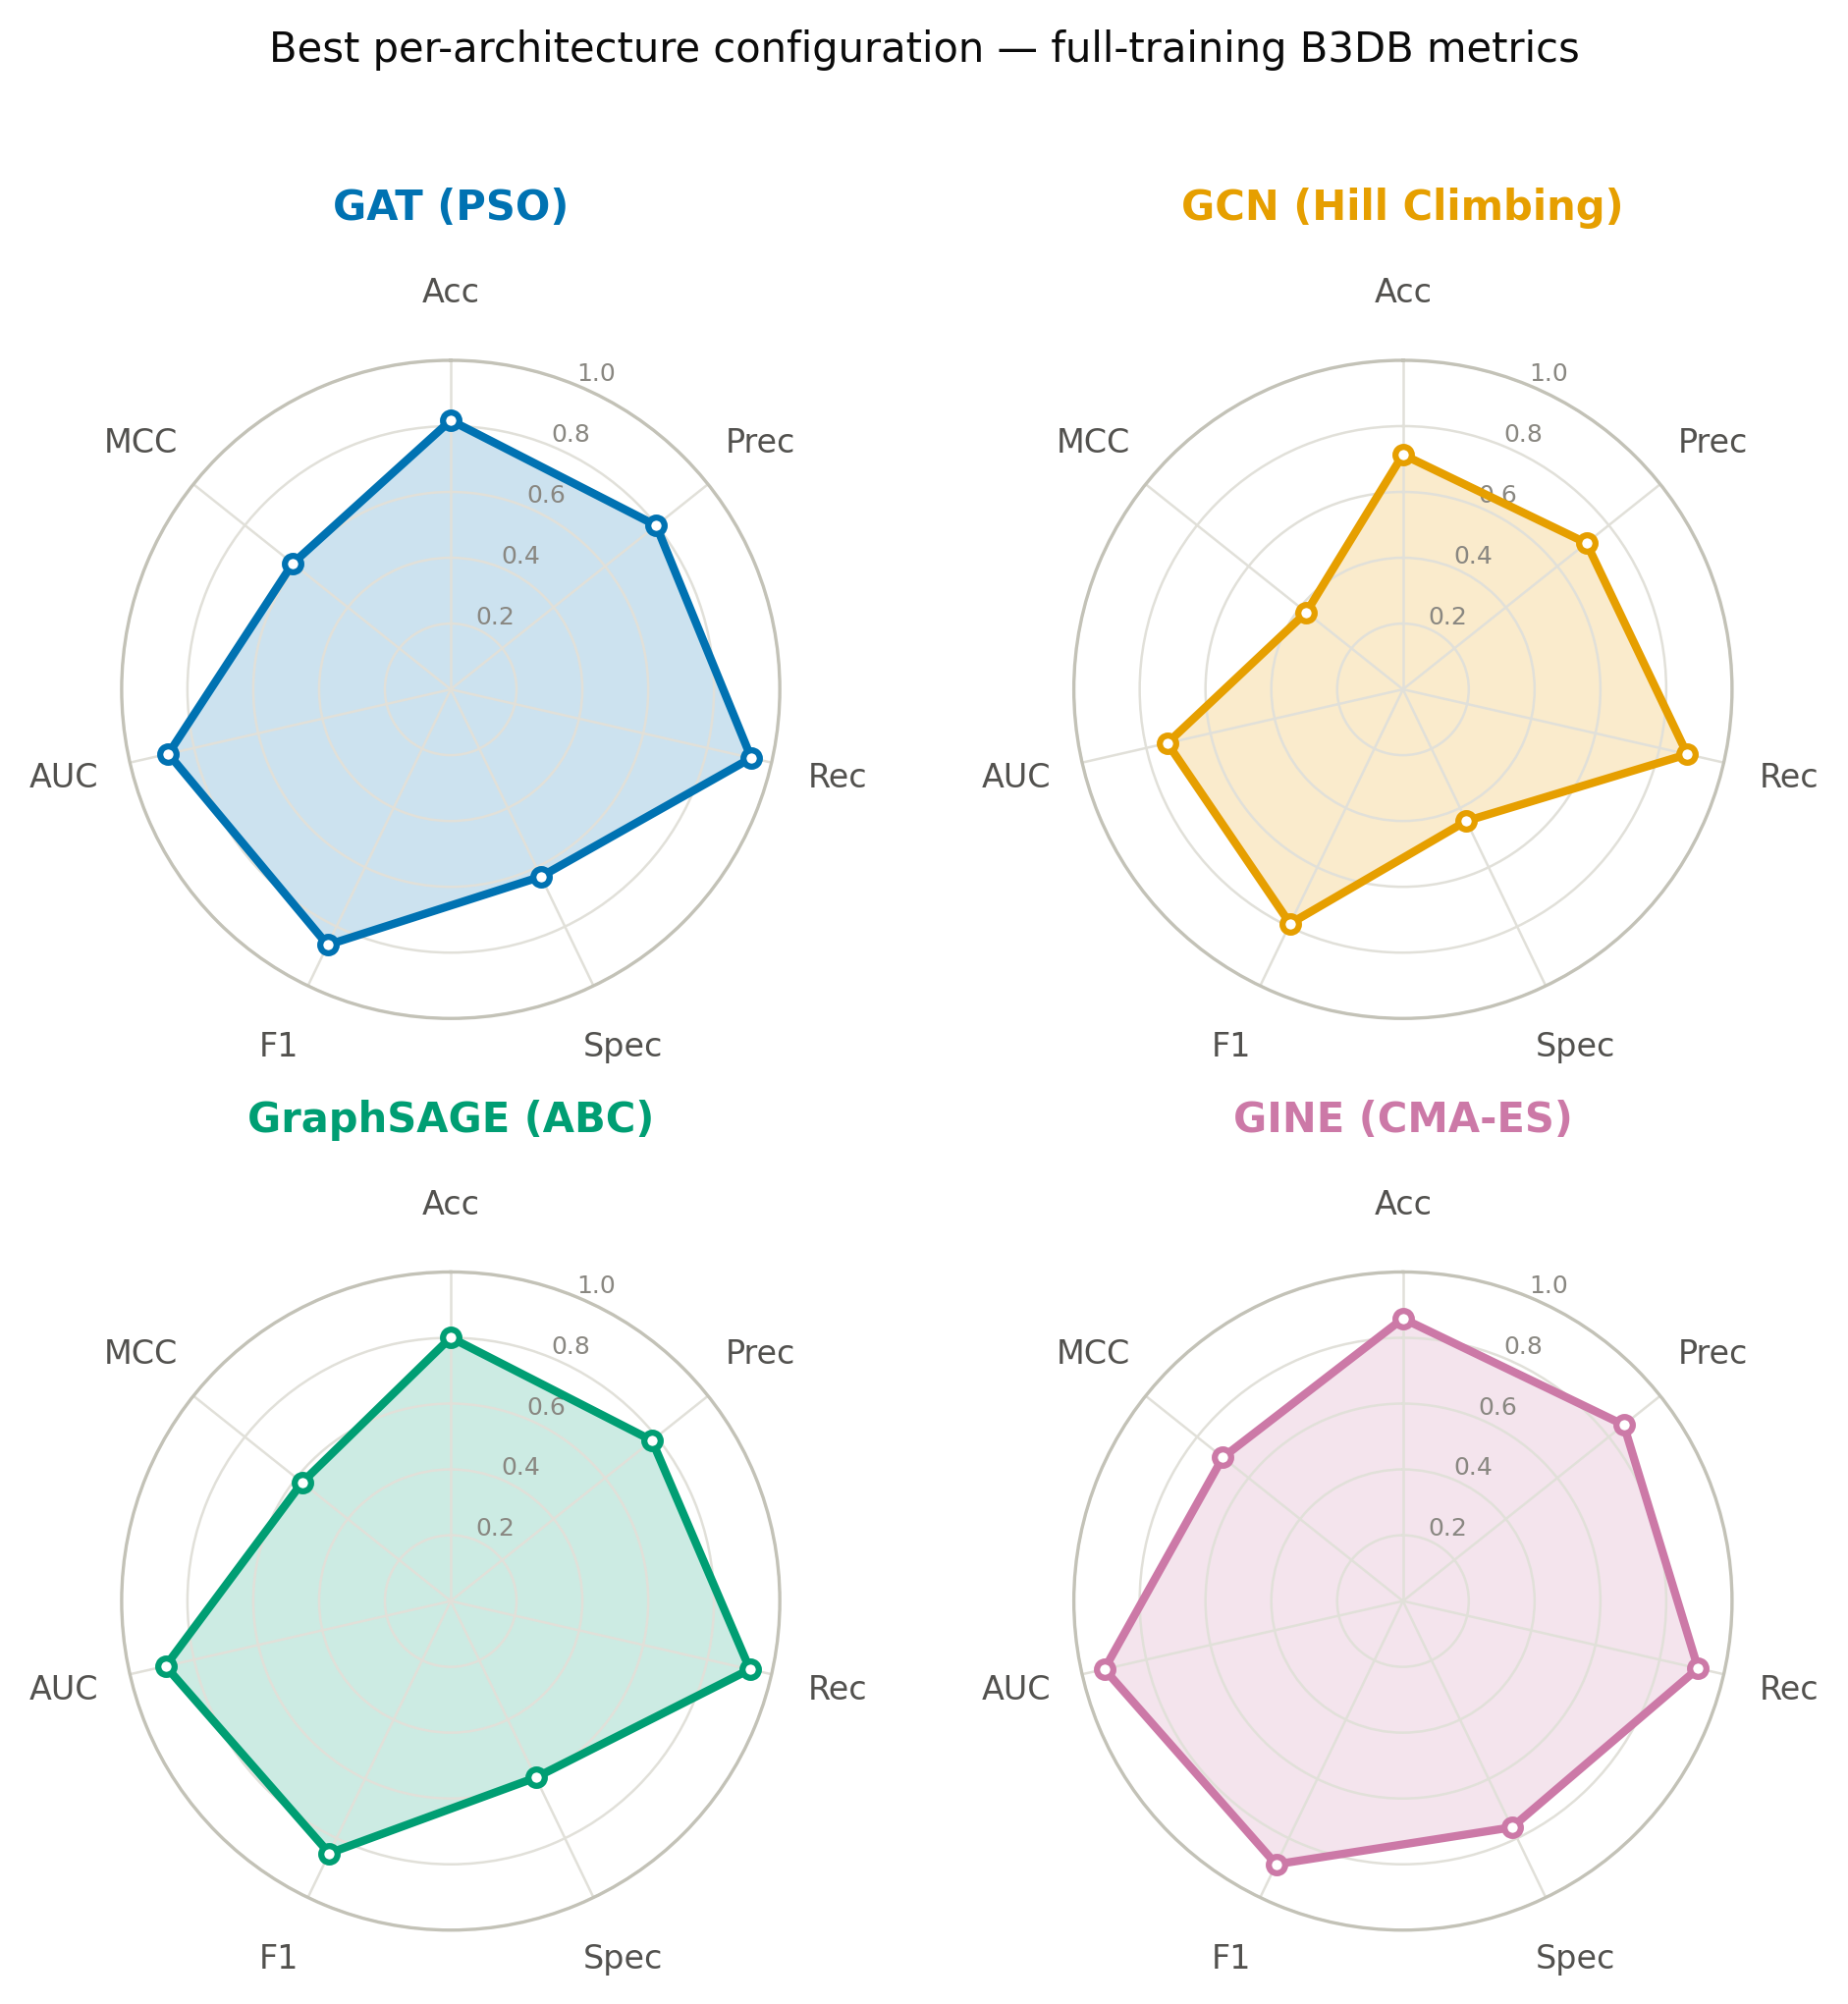
\includegraphics[width=\columnwidth]{fig2_radar_combined.png}
    \caption{Radar charts comparing seven performance metrics
             (accuracy, precision, recall, specificity, F1, AUC, MCC)
             for the best optimizer configuration per GNN architecture,
             trained on the full B3DB dataset for 100 epochs. A larger,
             more symmetrical polygon indicates stronger and more
             balanced performance. The contracted Spec axis in GCN and
             the elongated Rec axis in GAT expose the
             recall-specificity imbalance that F1 alone conceals.}
    \label{fig:radar}
\end{figure}

GINE emerged as the strongest architecture. CMA-ES achieved accuracy
0.8586, F1 0.8880, AUC 0.9307, and MCC 0.7000, with strong
specificity (0.7632) reflecting balanced discrimination of both
permeable and non-permeable compounds. GAT ranked second (PSO: F1
0.8621, MCC 0.6140), consistently achieving recall above 0.89 across
all optimizers but with comparatively lower specificity (0.54--0.64),
indicating a majority-class bias that the radar chart in
Fig.~\ref{fig:radar} makes visually apparent when comparing GAT's
shape against GINE's more balanced polygon. GraphSAGE (ABC: F1 0.8508,
AUC 0.8890) confirmed that mean neighborhood aggregation is
competitive with appropriate hyperparameters. GCN consistently
underperformed, with specificity as low as 0.2566 (Hyperband),
reflecting its limited native capacity to exploit bond-level edge
features.

\subsection{Cross-Dataset Generalization}

The best configuration per architecture, GAT (PSO), GCN (Hill
Climbing), GraphSAGE (ABC), and GINE (CMA-ES), was evaluated on
MoleculeNet and LCD, both held out entirely from training and
hyperparameter search. Fig.~\ref{fig:cross_dataset} reports ROC-AUC
and MCC across all three datasets. ROC-AUC is used because it is
threshold-independent and comparable across datasets with different
class distributions, particularly important given MoleculeNet's
heavier BBB$+$ imbalance relative to B3DB. MCC complements AUC by
quantifying whether absolute classification decisions hold under
distributional shift, penalizing models that maintain high F1 by
over-predicting the majority class.

\begin{figure*}[htbp]
    \centering
    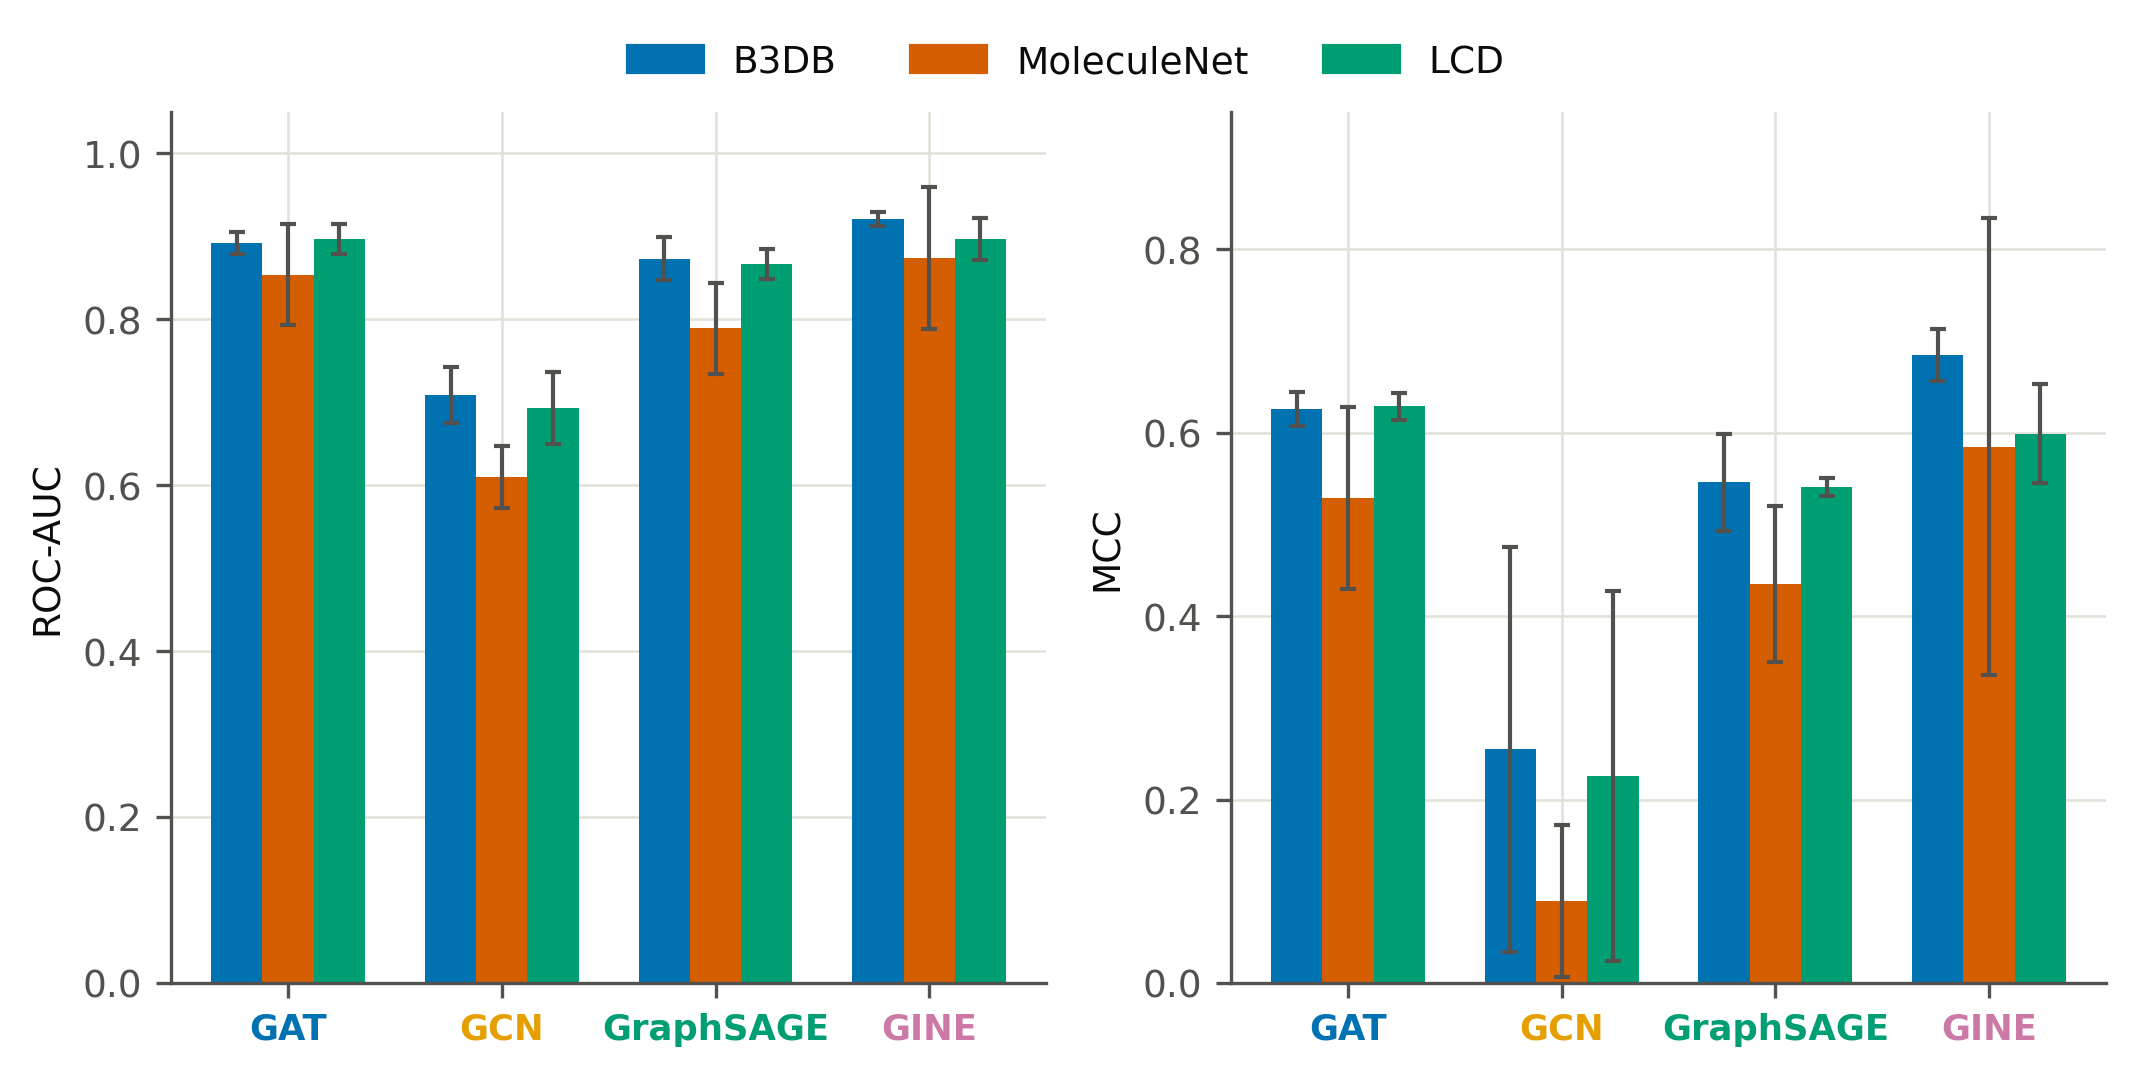
\includegraphics[width=\textwidth]{fig3_cross_dataset_generalization.png}
    \caption{Cross-dataset generalization of the best GNN configuration
             per architecture, measured by ROC-AUC (left) and MCC
             (right) across B3DB, MoleculeNet, and LCD. ROC-AUC
             is threshold-independent and remains comparable across
             datasets with differing class distributions. MCC captures
             whether absolute classification decisions hold under
             distributional shift, penalizing models that maintain
             high F1 by over-predicting the majority class.}
    \label{fig:cross_dataset}
\end{figure*}

GAT demonstrated the most consistent cross-dataset behavior (F1:
0.865$\pm$0.006, 0.874$\pm$0.018, 0.894$\pm$0.026 across B3DB,
MoleculeNet, LCD), with only a modest MCC decline on MoleculeNet
(0.626$\pm$0.019$\to$0.529$\pm$0.099) reflecting somewhat reduced
discrimination of BBB-negative compounds on the more imbalanced
external set. GCN exhibited the sharpest generalization decline: AUC
dropped from 0.709$\pm$0.034 to 0.610$\pm$0.037 and MCC from
0.255$\pm$0.221 to 0.089$\pm$0.083 on MoleculeNet, the largest
absolute drop among all four GNN architectures on both metrics, and
one that F1 alone would have masked (GCN's MoleculeNet F1 of
0.777$\pm$0.069 appears superficially competitive with its
B3DB performance). This divergence underscores why MCC is the more
reliable summary metric under class imbalance: F1 does not penalize a
model for systematically misclassifying the minority class, whereas
MCC does. GraphSAGE maintained F1 above 0.84 across all datasets with
moderate AUC degradation (0.873$\pm$0.026$\to$0.789$\pm$0.055 on
MoleculeNet). GINE also degrades notably on MoleculeNet (AUC:
0.921$\pm$0.009$\to$0.874$\pm$0.086; MCC:
0.685$\pm$0.028$\to$0.585$\pm$0.249), though its drop is smaller than
GCN's despite GINE's stronger in-distribution performance.

\subsection{Feature Analysis}
\label{sec:feature_analysis}

To assess what the best-performing model has learned and whether its
representations transfer across datasets, we visualise the graph-level
embeddings produced by GINE (CMA-ES) --- the GNN architecture with the
highest in-distribution MCC among the four studied here --- by
projecting them into two dimensions using
t-SNE (perplexity 40, 1,000 iterations) applied to the penultimate
layer activations.

The embedding coloured by BBB class (Fig.~\ref{fig:gin_embeddings},
left) reveals that GINE has learned a structured latent space with
appreciable BBB$+$/BBB$-$ separation, confirming that the model's
discriminative capacity is grounded in chemically meaningful
representations rather than superficial dataset artefacts. Colouring
by dataset and split membership (right) shows that B3DB training
molecules occupy the dense central region, while MoleculeNet and LCD
compounds populate peripheral sub-clusters. The overlap between
external-dataset compounds and the BBB$-$ boundary region provides a
geometric explanation for GINE's MCC collapse under distributional shift:
the model's decision boundary, optimised for B3DB's structural
distribution, does not generalise cleanly to the minority-class
molecules in the external sets.

% TODO(authors): replace gin_embeddings_tsne.png with the actual
% two-panel t-SNE projection (left: coloured by BBB class; right:
% coloured by dataset/split membership) referenced in this paragraph.
\begin{figure}[htbp]
    \centering
    \includegraphics[width=\columnwidth]{fig_gin_embeddings.png}
    \caption{t-SNE projection of GINE (CMA-ES) penultimate-layer graph
             embeddings, coloured by BBB class (left) and by dataset/split
             membership (right).}
    \label{fig:gin_embeddings}
\end{figure}

\subsection{Comparison with Baseline Models}

The best GNN configurations were compared against ten baseline models
on the B3DB test partition: three classical baselines trained in this
work (Logistic Regression, Random Forest, and XGBoost), plus seven
published models, LightBBB~\cite{Shaker2021} (which also stands in for
our reproduced LightGBM baseline; Section~\ref{sec:evaluation}),
DeePred-BBB~\cite{Kumar2022}, Deep-B3~\cite{Tang2022},
AttentiveFP~\cite{Xiong2020}, GROVER-BBBp~\cite{Tong2022},
ChemBERTa-FT~\cite{Ahmad2022chemberta2}, and
MolCLR~\cite{Wang2022molclr}. Results are in
Tables~\ref{tab:model_comparison_nongraph} and
\ref{tab:model_comparison_graph}. Fig.~\ref{fig:model_comparison}
ranks all models by AUC and MCC. AUC is threshold-independent
and directly comparable across datasets with differing class
distributions; MCC accounts for all four confusion matrix quadrants
and is the most informative single metric under class imbalance,
jointly penalizing false positives and false negatives including
compounds incorrectly identified as BBB-impermeable, whose
misclassification carries direct cost in drug discovery pipelines.

% Table 3a: full two-column (non-graph baselines)
\begin{table*}[htbp]
\caption{Performance Comparison of Non-Graph / Descriptor-Based Models on B3DB and External Datasets}
\label{tab:model_comparison_nongraph}
\centering
\footnotesize
\renewcommand{\arraystretch}{1.3}
\resizebox{\textwidth}{!}{%
\begin{tabular}{llccccccc}
\hline
\textbf{Model} & \textbf{Dataset} & \textbf{Acc} & \textbf{Prec} & \textbf{Rec} & \textbf{Spec} & \textbf{F1} & \textbf{AUC} & \textbf{MCC} \\
\hline
\multicolumn{9}{l}{\textit{In-house classical (Morgan fingerprints)}} \\
\hline
\multirow{3}{*}{Logistic Regression}
    & B3DB        & 0.802$\pm$0.000 & 0.838$\pm$0.000 & 0.838$\pm$0.000 & 0.746$\pm$0.000 & 0.838$\pm$0.000 & 0.883$\pm$0.000 & 0.584$\pm$0.001 \\
    & MoleculeNet & 0.793$\pm$0.000 & 0.838$\pm$0.000 & 0.884$\pm$0.000 & 0.561$\pm$0.000 & 0.860$\pm$0.000 & 0.806$\pm$0.000 & 0.467$\pm$0.000 \\
    & LCD      & 0.838$\pm$0.002 & 0.948$\pm$0.000 & 0.830$\pm$0.003 & 0.862$\pm$0.001 & 0.885$\pm$0.002 & 0.910$\pm$0.000 & 0.630$\pm$0.005 \\
\hline
\multirow{3}{*}{Random Forest}
    & B3DB        & 0.853$\pm$0.002 & 0.843$\pm$0.002 & 0.932$\pm$0.003 & 0.729$\pm$0.005 & 0.885$\pm$0.002 & 0.946$\pm$0.001 & 0.687$\pm$0.004 \\
    & MoleculeNet & 0.833$\pm$0.005 & 0.815$\pm$0.005 & 0.993$\pm$0.000 & 0.421$\pm$0.018 & 0.895$\pm$0.003 & 0.855$\pm$0.006 & 0.566$\pm$0.014 \\
    & LCD      & 0.941$\pm$0.007 & 0.954$\pm$0.011 & 0.968$\pm$0.008 & 0.859$\pm$0.035 & 0.961$\pm$0.004 & 0.974$\pm$0.000 & 0.840$\pm$0.020 \\
\hline
\multirow{3}{*}{XGBoost}
    & B3DB        & 0.847$\pm$0.005 & 0.837$\pm$0.006 & 0.930$\pm$0.000 & 0.716$\pm$0.012 & 0.881$\pm$0.003 & 0.927$\pm$0.001 & 0.675$\pm$0.010 \\
    & MoleculeNet & 0.844$\pm$0.011 & 0.837$\pm$0.008 & 0.973$\pm$0.007 & 0.515$\pm$0.027 & 0.900$\pm$0.007 & 0.842$\pm$0.004 & 0.591$\pm$0.034 \\
    & LCD      & 0.906$\pm$0.010 & 0.961$\pm$0.003 & 0.912$\pm$0.014 & 0.888$\pm$0.008 & 0.936$\pm$0.008 & 0.956$\pm$0.002 & 0.765$\pm$0.022 \\
\hline
\multicolumn{9}{l}{\textit{Published, descriptor-based}} \\
\hline
\multirow{3}{*}{LightBBB}
    & B3DB        & 0.8241 & 0.8248 & 0.9071 & 0.6923 & 0.8635 & 0.8711 & 0.6235 \\
    & MoleculeNet & 0.9701 & 0.9929 & 0.9653 & 0.9825 & 0.9789 & 0.9595 & 0.9291 \\
    & LCD      & 0.7739 & 0.9252 & 0.7596 & 0.8168 & 0.8343 & 0.7591 & 0.5136 \\
\hline
\multirow{3}{*}{DeePred-BBB}
    & B3DB        & 0.5944 & 0.7062 & 0.5888 & 0.6036 & 0.6421 & 0.3762      & 0.1870 \\
    & MoleculeNet & 0.4631 & 0.7126 & 0.4247 & 0.5614 & 0.5322 & 0.3919      & -0.0127 \\
    & LCD      & 0.4668 & 0.7650 & 0.4192 & 0.6107 & 0.5416 & 0.3295      & 0.0262 \\
\hline
\multicolumn{9}{l}{\textit{Published, non-graph language model}} \\
\hline
\multirow{3}{*}{ChemBERTa-FT}
    & B3DB        & 0.856$\pm$0.012 & 0.906$\pm$0.013 & 0.853$\pm$0.037 & 0.861$\pm$0.027 & 0.878$\pm$0.014 & 0.919$\pm$0.005 & 0.705$\pm$0.017 \\
    & MoleculeNet & 0.819$\pm$0.003 & 0.915$\pm$0.016 & 0.826$\pm$0.017 & 0.801$\pm$0.044 & 0.868$\pm$0.003 & 0.883$\pm$0.002 & 0.592$\pm$0.017 \\
    & LCD      & 0.848$\pm$0.016 & 0.960$\pm$0.011 & 0.832$\pm$0.031 & 0.893$\pm$0.035 & 0.891$\pm$0.014 & 0.937$\pm$0.002 & 0.660$\pm$0.017 \\
\hline
\multicolumn{9}{l}{\textit{External codebases, non-graph}} \\
\hline
\multirow{3}{*}{Classical ML Descriptor Models (RFC)}
    & B3DB        & 0.885$\pm$0.003 & 0.880$\pm$0.003 & 0.940$\pm$0.001 & 0.799$\pm$0.007 & 0.909$\pm$0.002 & 0.952$\pm$0.000 & 0.756$\pm$0.006 \\
    & MoleculeNet & 0.841$\pm$0.017 & 0.835$\pm$0.010 & 0.970$\pm$0.016 & 0.509$\pm$0.030 & 0.898$\pm$0.011 & 0.884$\pm$0.003 & 0.582$\pm$0.052 \\
    & LCD      & 0.923$\pm$0.003 & 0.975$\pm$0.004 & 0.922$\pm$0.003 & 0.929$\pm$0.012 & 0.948$\pm$0.002 & 0.978$\pm$0.001 & 0.810$\pm$0.008 \\
\hline
\multirow{3}{*}{VAE-Embeddings}
    & B3DB        & 0.825$\pm$0.007 & 0.831$\pm$0.006 & 0.895$\pm$0.005 & 0.716$\pm$0.011 & 0.862$\pm$0.005 & 0.909$\pm$0.005 & 0.628$\pm$0.015 \\
    & MoleculeNet & 0.805$\pm$0.003 & 0.805$\pm$0.013 & 0.961$\pm$0.024 & 0.403$\pm$0.063 & 0.876$\pm$0.003 & 0.795$\pm$0.024 & 0.474$\pm$0.006 \\
    & LCD      & 0.879$\pm$0.006 & 0.955$\pm$0.008 & 0.880$\pm$0.011 & 0.875$\pm$0.025 & 0.916$\pm$0.004 & 0.941$\pm$0.005 & 0.708$\pm$0.013 \\
\hline
\end{tabular}
}

\vspace{2pt}
{\footnotesize ChemBERTa-FT, Classical ML Descriptor Models (RFC),
VAE-Embeddings, and the in-house Logistic Regression, Random Forest, and
XGBoost baselines are reported as mean $\pm$ std over three random seeds
(the original seed plus two additional seeds); all other rows in this
table (LightBBB, DeePred-BBB) remain single-run point estimates.
Logistic Regression's B3DB/MoleculeNet standard deviations round to
0.000 at three decimal places because its lbfgs solver converges to
the same decision boundary regardless of \texttt{random\_state} on
this well-conditioned, linearly-separable-enough feature space: across
the three seeds, Precision/Recall/F1 are bit-identical predictions
(true std $=$ 0), while Accuracy, Specificity, AUC, and MCC vary by
$<$0.0006 (e.g.\ B3DB MCC std $\approx$0.00052), i.e.\ genuinely
near-zero rather than exactly zero. Only the LCD (sdata) evaluation
shows more than rounding-level seed sensitivity.
LightBBB was evaluated through its public web interface rather than a
locally reproducible pipeline, so no reproduction script or checkpoint
exists in our codebase and its numbers could not be independently
regenerated or re-seeded. DeePred-BBB, by contrast, is reproduced
locally: it is deterministic inference against a fixed pretrained
checkpoint we hold with no training step, so re-running it under a
different seed would not change its results. See notes.md for details.}
\end{table*}

% Table 3b: full two-column (graph-based baselines)
\begin{table*}[htbp]
\caption{Performance Comparison of Graph-Based Models on B3DB and External Datasets}
\label{tab:model_comparison_graph}
\centering
\footnotesize
\renewcommand{\arraystretch}{1.3}
\begin{tabular}{llccccccc}
\hline
\textbf{Model} & \textbf{Dataset} & \textbf{Acc} & \textbf{Prec} & \textbf{Rec} & \textbf{Spec} & \textbf{F1} & \textbf{AUC} & \textbf{MCC} \\
\hline
\multicolumn{9}{l}{\textit{Published, graph-based}} \\
\hline
\multirow{3}{*}{Deep-B3}
    & B3DB        & 0.8329 & 0.8426 & 0.8924 & 0.7401 & 0.8668 & 0.8744 & 0.6450 \\
    & MoleculeNet & 0.9015 & 0.9632 & 0.8973 & 0.9123 & 0.9291 & 0.9048 & 0.7737 \\
    & LCD      & 0.7989 & 0.9613 & 0.7621 & 0.9084 & 0.8502 & 0.8127 & 0.5920 \\
\hline
\multirow{3}{*}{AttentiveFP}
    & B3DB        & 0.7771 & 0.7935 & 0.9325 & 0.6217 & 0.8573 & 0.8705 & 0.5996 \\
    & MoleculeNet & 0.8460 & 0.8987 & 0.9726 & 0.7193 & 0.9344 & 0.9567 & 0.7486 \\
    & LCD      & 0.8150 & 0.9020 & 0.9276 & 0.7023 & 0.9146 & 0.9195 & 0.6490 \\
\hline
\multirow{3}{*}{GROVER-BBBp}
    & B3DB        & 0.7906 & 0.8025 & 0.9430 & 0.6382 & 0.8670 & 0.8877 & 0.6288 \\
    & MoleculeNet & 0.9581 & 0.9730 & 0.9863 & 0.9298 & 0.9794 & 0.9921 & 0.9263 \\
    & LCD      & 0.8144 & 0.8967 & 0.9646 & 0.6641 & 0.9289 & 0.9211 & 0.6904 \\
\hline
\multirow{3}{*}{MolCLR}
    & B3DB        & 0.836$\pm$0.004 & 0.867$\pm$0.005 & 0.863$\pm$0.015 & 0.794$\pm$0.013 & 0.865$\pm$0.005 & 0.915$\pm$0.001 & 0.656$\pm$0.006 \\
    & MoleculeNet & 0.814$\pm$0.008 & 0.854$\pm$0.011 & 0.895$\pm$0.004 & 0.608$\pm$0.037 & 0.874$\pm$0.004 & 0.840$\pm$0.008 & 0.525$\pm$0.025 \\
    & LCD      & 0.849$\pm$0.003 & 0.964$\pm$0.002 & 0.830$\pm$0.004 & 0.906$\pm$0.004 & 0.892$\pm$0.002 & 0.938$\pm$0.001 & 0.665$\pm$0.005 \\
\hline
\multicolumn{9}{l}{\textit{External codebases, graph-based}} \\
\hline
\multirow{3}{*}{Atom-Attention-MPNN}
    & B3DB        & 0.855$\pm$0.003 & 0.859$\pm$0.009 & 0.912$\pm$0.009 & 0.766$\pm$0.020 & 0.885$\pm$0.002 & 0.935$\pm$0.001 & 0.693$\pm$0.007 \\
    & MoleculeNet & 0.839$\pm$0.006 & 0.832$\pm$0.010 & 0.973$\pm$0.014 & 0.497$\pm$0.041 & 0.897$\pm$0.003 & 0.879$\pm$0.002 & 0.578$\pm$0.018 \\
    & LCD      & 0.875$\pm$0.022 & 0.966$\pm$0.004 & 0.864$\pm$0.034 & 0.908$\pm$0.015 & 0.912$\pm$0.017 & 0.951$\pm$0.003 & 0.713$\pm$0.033 \\
\hline
\multirow{3}{*}{RGCN}
    & B3DB        & 0.870$\pm$0.015 & 0.886$\pm$0.009 & 0.904$\pm$0.021 & 0.818$\pm$0.016 & 0.894$\pm$0.013 & 0.939$\pm$0.001 & 0.726$\pm$0.030 \\
    & MoleculeNet & 0.841$\pm$0.010 & 0.852$\pm$0.018 & 0.943$\pm$0.014 & 0.579$\pm$0.063 & 0.895$\pm$0.006 & 0.882$\pm$0.016 & 0.583$\pm$0.031 \\
    & LCD      & 0.890$\pm$0.008 & 0.926$\pm$0.009 & 0.928$\pm$0.023 & 0.776$\pm$0.035 & 0.927$\pm$0.007 & 0.940$\pm$0.004 & 0.706$\pm$0.011 \\
\hline
\multicolumn{9}{l}{\textit{GNN architectures optimized in this study (mean $\pm$ std, $n=3$ seeds)}} \\
\hline
\multirow{3}{*}{GAT}
    & B3DB        & 0.824$\pm$0.009 & 0.813$\pm$0.014 & 0.924$\pm$0.012 & 0.668$\pm$0.033 & 0.865$\pm$0.006 & 0.892$\pm$0.013 & 0.626$\pm$0.019 \\
    & MoleculeNet & 0.815$\pm$0.030 & 0.860$\pm$0.048 & 0.890$\pm$0.045 & 0.620$\pm$0.172 & 0.874$\pm$0.018 & 0.854$\pm$0.061 & 0.529$\pm$0.099 \\
    & LCD         & 0.848$\pm$0.025 & 0.873$\pm$0.065 & 0.919$\pm$0.024 & 0.694$\pm$0.071 & 0.894$\pm$0.026 & 0.897$\pm$0.018 & 0.629$\pm$0.015 \\
\hline
\multirow{3}{*}{GCN}
    & B3DB        & 0.680$\pm$0.061 & 0.689$\pm$0.071 & 0.899$\pm$0.095 & 0.337$\pm$0.298 & 0.775$\pm$0.017 & 0.709$\pm$0.034 & 0.255$\pm$0.221 \\
    & MoleculeNet & 0.670$\pm$0.055 & 0.747$\pm$0.032 & 0.831$\pm$0.183 & 0.257$\pm$0.273 & 0.777$\pm$0.069 & 0.610$\pm$0.037 & 0.089$\pm$0.083 \\
    & LCD         & 0.729$\pm$0.020 & 0.778$\pm$0.046 & 0.861$\pm$0.121 & 0.368$\pm$0.321 & 0.813$\pm$0.044 & 0.693$\pm$0.043 & 0.226$\pm$0.202 \\
\hline
\multirow{3}{*}{GraphSAGE}
    & B3DB        & 0.787$\pm$0.024 & 0.772$\pm$0.023 & 0.923$\pm$0.008 & 0.575$\pm$0.054 & 0.841$\pm$0.016 & 0.873$\pm$0.026 & 0.546$\pm$0.053 \\
    & MoleculeNet & 0.787$\pm$0.022 & 0.823$\pm$0.036 & 0.900$\pm$0.031 & 0.497$\pm$0.142 & 0.859$\pm$0.011 & 0.789$\pm$0.055 & 0.435$\pm$0.085 \\
    & LCD         & 0.822$\pm$0.029 & 0.833$\pm$0.049 & 0.931$\pm$0.011 & 0.558$\pm$0.027 & 0.879$\pm$0.032 & 0.867$\pm$0.018 & 0.541$\pm$0.010 \\
\hline
\multirow{3}{*}{GINE}
    & B3DB        & 0.852$\pm$0.013 & 0.855$\pm$0.018 & 0.912$\pm$0.007 & 0.758$\pm$0.035 & 0.882$\pm$0.009 & 0.921$\pm$0.009 & 0.685$\pm$0.028 \\
    & MoleculeNet & 0.842$\pm$0.087 & 0.870$\pm$0.078 & 0.922$\pm$0.028 & 0.637$\pm$0.239 & 0.895$\pm$0.054 & 0.874$\pm$0.086 & 0.585$\pm$0.249 \\
    & LCD         & 0.831$\pm$0.004 & 0.883$\pm$0.053 & 0.886$\pm$0.055 & 0.729$\pm$0.077 & 0.880$\pm$0.006 & 0.897$\pm$0.025 & 0.599$\pm$0.054 \\
\hline
\end{tabular}

\vspace{2pt}
{\footnotesize Atom-Attention-MPNN's evaluation pipeline does not
natively compute F1 or MCC; both are computed directly from the
ensemble's predicted probabilities (thresholded at 0.5) against the
true labels, matching the Acc/Prec/Rec/Spec/AUC reported by the
codebase's own chemprop-based evaluation on the same predictions.
Atom-Attention-MPNN, RGCN, MolCLR, and
our four GNN architectures (GAT, GCN, GraphSAGE, GINE) are reported as
mean $\pm$ std over three random seeds; for the four GNN architectures,
each is the best-per-architecture configuration
(Section~\ref{sec:hpo_methods}) retrained end-to-end for three random
seeds (the original seed plus two additional seeds), and for
Atom-Attention-MPNN/RGCN/MolCLR the same three-seed protocol is applied
to the externally developed codebase without modification. All other
rows in this table remain single-run point estimates. GCN's large
standard deviations, and in particular an MCC of 0 for one seed,
reflect a collapse to majority-class prediction on that run rather
than a computation error, consistent with GCN's comparatively weak and
seed-sensitive specificity already noted in Section~\ref{sec:full_training_eval}.
Deep-B3 was evaluated through its public web interface rather than a
locally reproducible pipeline, so no reproduction script or checkpoint
exists in our codebase and its numbers could not be independently
regenerated or re-seeded. AttentiveFP and GROVER-BBBp, by contrast, are
reproduced locally here: both perform deterministic inference against a
fixed pretrained checkpoint we hold rather than training from
scratch, so re-running them under a different seed would not change their
results; their rows remain single-run point estimates. See notes.md for
details on all three.}
\end{table*}

\begin{figure*}[htbp]
    \centering
    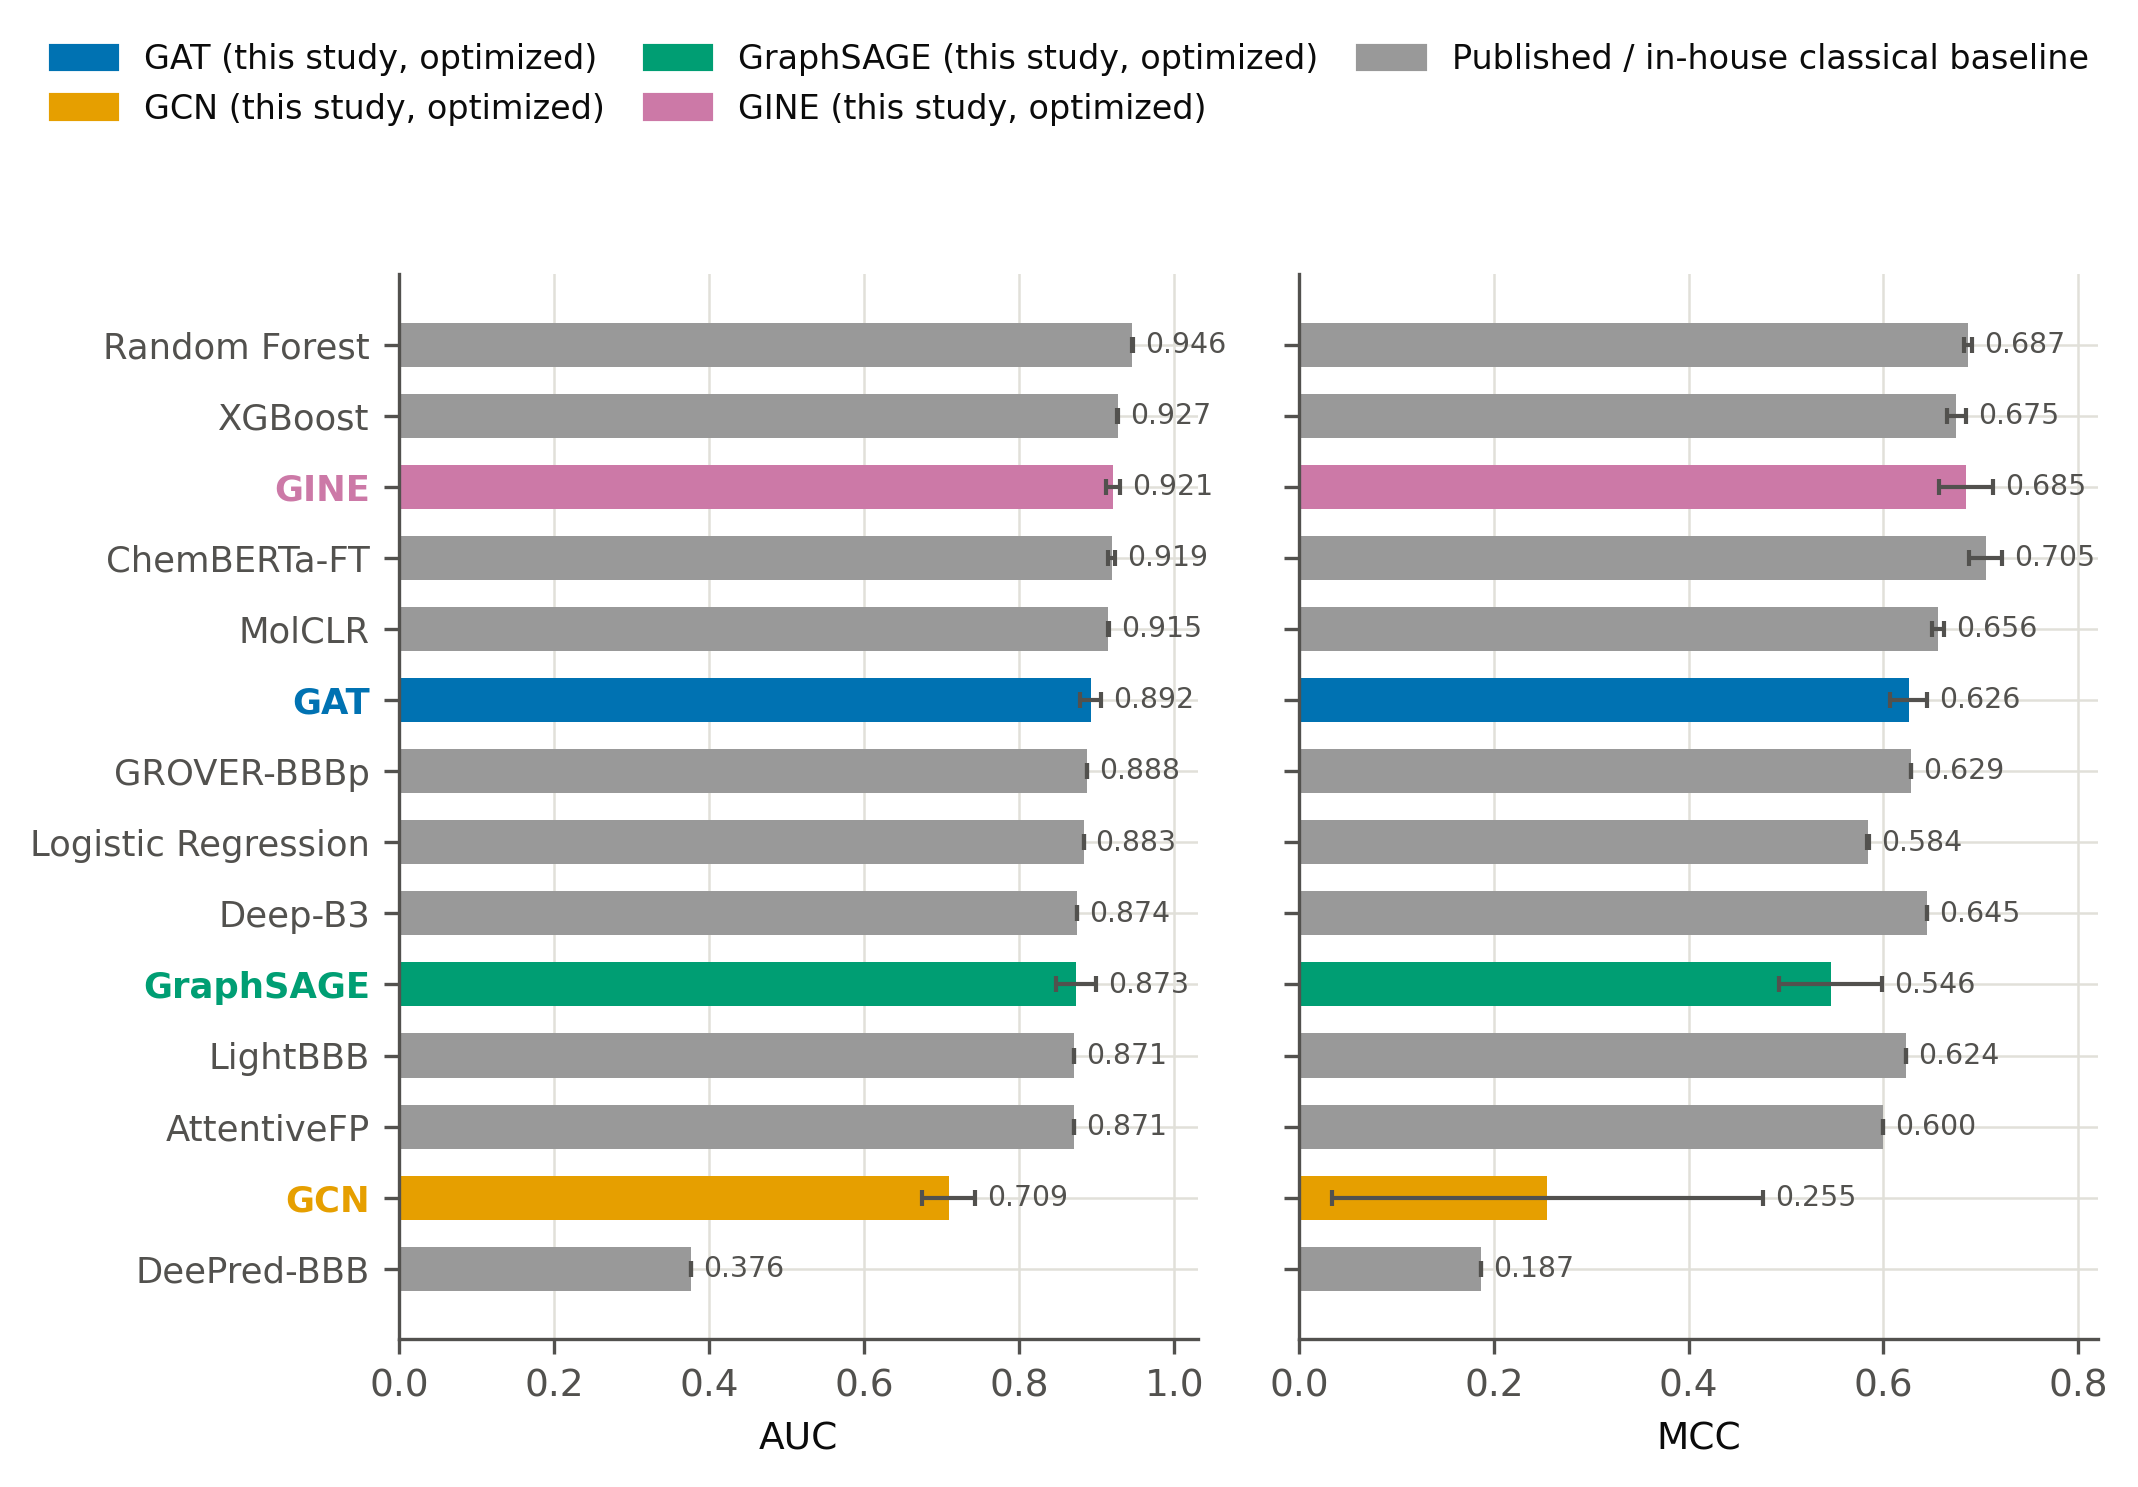
\includegraphics[width=\textwidth]{fig4_model_comparison_b3db.png}
    \caption{Ranking of our four GNN architectures, three in-house
             classical baselines, and seven published models on the
             B3DB test set by AUC (upper bar) and MCC (lower bar),
             sorted in descending order of AUC (the four additional
             external codebases of Section~\ref{sec:additional_codebases_results}
             are evaluated separately and are not depicted here). GNN models (GAT,
             GCN, GraphSAGE, GINE) are shown in distinct colours (blue,
             orange, green, purple respectively); published baseline
             models are shown in grey. Among the models shown, Random
             Forest achieves the highest AUC (0.946), while GINE leads
             among GNN architectures (AUC\,=\,0.921$\pm$0.009, MCC\,=\,0.685$\pm$0.028);
             Classical ML Descriptor Models (RFC) (Table~\ref{tab:model_comparison_nongraph}) and RGCN (Table~\ref{tab:model_comparison_graph})
             exceed both on AUC and MCC but are outside the scope of
             this figure. DeePred-BBB is the weakest performer among
             the models shown, with an AUC of 0.376 and an MCC of
             0.187. AUC is threshold-independent and comparable across
             datasets with differing class distributions; MCC is
             the more informative metric under class imbalance,
             jointly accounting for true negatives---compounds
             correctly identified as BBB-impermeable---whose
             misclassification carries direct cost in drug
             discovery pipelines.}
    \label{fig:model_comparison}
\end{figure*}

Notably, Random Forest (AUC\,=\,0.946$\pm$0.001, MCC\,=\,0.687$\pm$0.004) achieves the
highest AUC among our four GNN architectures, the three classical
baselines, and the seven published models compared in this subsection,
reinforcing that well-tuned descriptor-based methods remain highly
competitive on in-distribution data. XGBoost (AUC\,=\,0.927$\pm$0.001,
MCC\,=\,0.675$\pm$0.010) similarly matches GINE on MCC while demonstrating
stronger cross-dataset F1 on MoleculeNet (0.900$\pm$0.007). GINE (CMA-ES)
nonetheless leads all four GNN architectures on F1 (0.882$\pm$0.009) and
achieves the highest GNN MCC (0.685$\pm$0.028), surpassing six of the seven
published baselines. (Section~\ref{sec:additional_codebases_results}
below extends this comparison further with four additional external
codebases, two of which exceed GINE on F1, AUC, and MCC.) However,
ChemBERTa-FT (MCC\,=\,0.705$\pm$0.017, F1\,=\,0.878$\pm$0.014, AUC\,=\,0.919$\pm$0.005)
narrowly outperforms GINE on MCC, emerging as the strongest published
baseline in this comparison. ChemBERTa-FT also achieves
the highest precision (0.906$\pm$0.013) and specificity (0.861$\pm$0.027) among all
evaluated models, indicating well-balanced discrimination with few
false-positive BBB predictions. MolCLR (MCC\,=\,0.656$\pm$0.006, F1\,=\,0.865$\pm$0.005,
AUC\,=\,0.915$\pm$0.001) exceeds GINE on specificity (0.794$\pm$0.013 vs.\
0.758$\pm$0.035), suggesting
that contrastive pre-training strategies confer a measurable advantage
in minority-class identification. Together, Random Forest, XGBoost,
ChemBERTa-FT, and MolCLR extend the finding that strong non-GNN and
pre-trained baselines remain highly competitive, and in several cases
can match or surpass the best-tuned GNN on key summary metrics.

GINE's MCC lead over the remaining published baselines (next best:
MolCLR, 0.656$\pm$0.006) still reflects genuinely better balanced
discrimination than the majority of the field. GAT (PSO) and
GraphSAGE (ABC) achieved F1 scores comparable to GROVER-BBBp (0.8670)
and AttentiveFP (0.8573), but their lower MCC values (0.626$\pm$0.019 and
0.546$\pm$0.053) reveal a high-recall, low-specificity bias. LightBBB
(F1\,=\,0.8635, MCC\,=\,0.6235) remained a strong competitor despite
using only handcrafted descriptors, confirming the systematic review
finding that well-tuned non-GNN models remain highly competitive.
DeePred-BBB (F1\,=\,0.6421) was the weakest model overall.

\subsection{Comparison with Additional External Codebases}
\label{sec:additional_codebases_results}

To extend this comparison beyond in-house baselines and the published
literature, we evaluated four additional externally developed
BBB-prediction codebases (Section~IV-F) under the identical
Tanimoto-based B3DB/MoleculeNet/LCD protocol; results appear in the
rows labeled ``External codebases'' within
Table~\ref{tab:model_comparison_nongraph} (Classical ML Descriptor
Models (RFC) and VAE-Embeddings) and
Table~\ref{tab:model_comparison_graph} (Atom-Attention-MPNN and RGCN). Classical ML Descriptor Models
(RFC), trained on Mordred 2D descriptors rather than Morgan
fingerprints, achieves the highest AUC (0.952$\pm$0.000) and highest MCC
(0.756$\pm$0.006) of every model evaluated in this study on B3DB, exceeding
both our in-house Random Forest (AUC\,=\,0.946$\pm$0.001) and the previously
best-placed published baseline, ChemBERTa-FT (MCC\,=\,0.705$\pm$0.017). This
result reflects the richer descriptor
set Mordred provides (we did not measure comparative feature-generation
runtime, so no claim about relative computational cost is made) rather
than a fundamentally stronger classifier,
since the underlying algorithm (Random Forest) is the same family
already represented in our own baselines. RGCN (AUC\,=\,0.939$\pm$0.001,
MCC\,=\,0.726$\pm$0.030 on B3DB) and Atom-Attention-MPNN (AUC\,=\,0.935$\pm$0.001,
F1\,=\,0.885$\pm$0.002) both perform competitively with GINE despite using default
hyperparameters rather than the seven-algorithm HPO sweep applied to
our own GNNs. VAE-Embeddings, the lightest-weight of the four (a
shallow MLP on fixed fingerprints, without the pretrained VAE encoder),
trails the others on B3DB (AUC\,=\,0.909$\pm$0.005, MCC\,=\,0.628$\pm$0.015) but achieves
its strongest relative result on LCD (AUC\,=\,0.941$\pm$0.005). All four
models reproduce the same generalization pattern already observed for
GINE and RandomForest: specificity drops sharply on MoleculeNet relative
to B3DB or LCD (e.g., Classical ML Descriptor Models (RFC): 0.799$\pm$0.007$\to$0.509$\pm$0.030; RGCN:
0.818$\pm$0.016$\to$0.579$\pm$0.063), confirming that MoleculeNet's heavier class
imbalance, rather than any single architecture's weakness, is the
dominant driver of cross-dataset MCC degradation across model
families.

% =====================================================================
%  VI. DISCUSSION
% =====================================================================
\section{Discussion}

\subsection{GNN Architecture and Optimization}

GINE's sum-based aggregation and Weisfeiler-Lehman expressive power make it the strongest architecture for BBB prediction on B3DB when paired with appropriate hyperparameter optimization. Its dedicated bond encoder enables fine-grained chemical discrimination that GCN's scalar edge weights and GraphSAGE's additive injection cannot match. CMA-ES performed particularly well for GINE: its covariance-adaptation mechanism is well-suited to non-convex hyperparameter landscapes, and it consistently identified configurations with both high performance and lower generalization gaps compared to alternative population-based optimizers such as PSO.

Across all optimizer configurations, GAT showed consistently low specificity. Its attention mechanism appears to amplify sensitivity toward the BBB$+$ majority class, producing high recall at the cost of true negative identification. This pattern likely reflects class imbalance in B3DB and suggests that attention-based architectures may benefit from class-weighted loss or explicit minority-class augmentation in future work.

\subsection{Generalization and Dataset Shift}

Cross-dataset evaluation shows that strong in-distribution performance does not reliably transfer under distributional shift. GINE's AUC and MCC drop sharply on MoleculeNet (AUC: 0.921$\pm$0.009$\to$0.874$\pm$0.086; MCC: 0.685$\pm$0.028$\to$0.585$\pm$0.249) despite a superficially competitive F1 (0.895$\pm$0.054), illustrating precisely why reporting F1 alone in BBB prediction papers is insufficient. Models that achieve high F1 under distributional shift may do so simply by predicting the majority class, a failure mode that MCC exposes immediately. The discrepancy between GINE's in-distribution and external MCC scores suggests possible overfitting to B3DB-specific structural patterns, which limits deployment reliability across chemical libraries with different composition.

GAT's cross-dataset consistency aligns with the systematic review finding that attention-based GNNs generalize more robustly on chemically diverse external sets. The attention mechanism's adaptive aggregation may act as an implicit regularizer, reducing over-reliance on substructural patterns present in B3DB but absent in MoleculeNet or LCD.

\subsection{Non-GNN Baselines Remain Competitive}

Random Forest (AUC\,=\,0.946$\pm$0.001) and XGBoost (MCC\,=\,0.675$\pm$0.010), trained
here on Morgan fingerprints, outperform or match GINE on several key
metrics, while LightBBB (F1\,=\,0.8635, MCC\,=\,0.6235) further
confirms that well-tuned descriptor-based methods remain highly
competitive. ChemBERTa-FT~\cite{Ahmad2022chemberta2} and
MolCLR~\cite{Wang2022molclr} strengthen this finding further.
ChemBERTa-FT (MCC\,=\,0.705$\pm$0.017), a fine-tuned chemical language model,
surpasses GINE~(CMA-ES) on MCC while matching it on F1, and MolCLR
(MCC\,=\,0.656$\pm$0.006), trained via contrastive learning on unlabeled
molecular data, exceeds all four GNNs on specificity. These results
are consistent with the systematic review finding that GNN advantages
are task-dependent rather than universal. GNNs are preferable primarily
in tasks requiring fine-grained structural discrimination, such as
stereochemical differentiation or active transport modeling. For tasks
where large pre-trained representations or handcrafted descriptors
capture the relevant chemical signals, non-GNN methods offer a
competitive and often more computationally efficient alternative.

\subsection{Additional External Codebases}

The four additional codebases evaluated in
Section~\ref{sec:additional_codebases_results} reinforce and
extend this pattern. Classical ML Descriptor Models (RFC) outperforming every model in
this study, including our own tuned GNNs and all seven published
baselines, on both AUC and MCC is best attributed to its Mordred
descriptor set rather than to Random Forest itself being a superior
algorithm to our in-house implementation: Mordred computes a
substantially larger and more chemically informative battery of 2D
descriptors than the 2048-bit Morgan fingerprints used elsewhere in
this study, and feature quality evidently mattered more here than
model architecture. This strengthens, rather than contradicts, the
systematic review's central finding that non-GNN approaches remain
highly competitive, and further suggests that descriptor engineering
is an underexplored lever in BBB prediction relative to the attention
paid to model architecture in the recent literature. RGCN and
Atom-Attention-MPNN closing most of the gap to our extensively
HPO-tuned GINE while using only default hyperparameters suggests that
message-passing architectures are comparatively robust to
hyperparameter choice on this task, though we cannot rule out that
targeted optimization of these two codebases would widen or close this
gap further. VAE-Embeddings' weaker performance is best interpreted as
a limitation of this evaluation rather than of the underlying
architecture: without the pretrained variational autoencoder
checkpoint, the model reduces to a shallow MLP on fixed fingerprints,
forgoing the learned representations the original architecture is
designed to provide.

% =====================================================================
%  VII. CONCLUSIONS
% =====================================================================
\section{Conclusions}

This paper reports a two-part investigation of BBB permeability prediction using graph neural networks. The systematic review of 26 studies established that GNN-based models offer advantages over non-GNN approaches primarily in structurally complex prediction scenarios, while non-GNN baselines remain highly competitive for passive diffusion prediction and offer superior computational efficiency and interpretability.

On the full B3DB benchmark, GINE optimized with CMA-ES achieved the
highest F1, AUC, and MCC among the four GNN architectures developed
and optimized in this study (F1\,=\,0.882$\pm$0.009, AUC\,=\,0.921$\pm$0.009,
MCC\,=\,0.685$\pm$0.028). Extending the comparison to four additional externally
developed BBB-prediction codebases evaluated under the identical
protocol, Classical ML Descriptor Models (Random Forest on Mordred descriptors) achieved
the highest F1 (0.909$\pm$0.002), AUC (0.952$\pm$0.000), and MCC (0.756$\pm$0.006) of every model
evaluated in this study, ahead of both our in-house Random Forest
(AUC\,=\,0.946$\pm$0.001) and the strongest published baseline,
ChemBERTa-FT~\cite{Ahmad2022chemberta2} (MCC\,=\,0.705$\pm$0.017). RGCN
(F1\,=\,0.894$\pm$0.013, AUC\,=\,0.939$\pm$0.001, MCC\,=\,0.726$\pm$0.030) also surpassed GINE on all
three summary metrics despite using default hyperparameters rather
than the seven-algorithm HPO sweep applied to our own GNNs. These
results indicate that both a richer descriptor set (Mordred) and an
externally developed message-passing architecture (RGCN) using only
default hyperparameters can match or exceed an extensively
hyperparameter-tuned bespoke GNN, reinforcing that classical and
off-the-shelf baselines remain formidable competitors under
Tanimoto-based evaluation. Hyperparameter
optimization analysis showed that high proxy validation F1 is not a
reliable indicator of proxy holdout performance, with generalization
gaps exceeding 0.17 in some optimizer-model combinations. Cross-dataset evaluation exposed a
critical limitation: GINE's in-distribution performance degrades
markedly under distributional shift (MCC: 0.685$\pm$0.028$\to$0.585$\pm$0.249 on
MoleculeNet), while GAT, despite ranking second among our own GNNs on
B3DB, maintains the most consistent performance across datasets.

The primary practical recommendation from this study is that BBB prediction models should be evaluated using MCC rather than F1 alone, as F1 can mask minority-class failures with direct consequences in drug discovery. Furthermore, Tanimoto-based data splitting is preferable to random splits to avoid inflated performance estimates.

% =====================================================================
%  VIII. LIMITATIONS AND FUTURE WORK
% =====================================================================
\section{Limitations and Future Work}

\subsection{Limitations}

Several limitations of this study should be acknowledged. First,
the experimental evaluation is restricted to four GNN architectures;
more recent models such as graph transformer architectures or
contrastive-pretraining-enhanced GNNs~\cite{Koutroumpa2025} were not
included in the empirical comparison.
Second, all GNN models were evaluated on a single primary benchmark
(B3DB), and while two external datasets were used for generalization
testing, the relatively small size of LCD (527 molecules) limits
the statistical confidence of those comparisons. Third, the
hyperparameter optimization proxy (10\% data, 10 epochs) may not
perfectly preserve the relative performance rankings observed under
full training, introducing a potential selection bias in the final
configurations. Fourth, the molecular graph representation does not
incorporate 3D conformational features
or protein–ligand interaction data, which are known to influence
active BBB transport mechanisms~\cite{Ding2022}. Finally, the
systematic review is limited to English-language publications in three
databases, and may not capture all relevant work in the field.

\subsection{Future Work}

Several directions emerge from this study. First, integrating 3D
molecular geometry and protein–ligand interaction data into the
graph representation could improve prediction of active transport
mechanisms, which current 2D GNNs inadequately model. Second,
developing contrastive or self-supervised pretraining strategies for
GCN and GINE may address the generalization gap observed on
MoleculeNet, particularly pronounced for GCN, by
leveraging large unlabeled molecular corpora to learn transferable
representations~\cite{Koutroumpa2025}. Third, exploring class-weighted
loss functions, focal loss, or explicit minority-class augmentation
could mitigate the specificity deficit observed in GAT and GraphSAGE.
Fourth, future work should investigate whether model ensembling,
for example, combining GINE's in-distribution discriminative power with
GAT's cross-dataset stability, produces a superior trade-off between
performance and generalization. Finally, extending the evaluation to
include unbound brain concentration prediction ($K_{p,uu}$) rather
than binary penetration classification would improve the biological
fidelity and translational value of computational BBB
models~\cite{Cornelissen2023}.


\nocite{*}
\bibliography{references}

\end{document}